    \documentclass[12pt]{article}
\usepackage{tocloft}
\usepackage{natbib}
\usepackage{url}
\usepackage[utf8x]{inputenc}
\usepackage{amsmath}
\usepackage{graphicx}
\usepackage{verbatim}
\graphicspath{{images/}}
\usepackage{parskip}
\usepackage{fancyhdr}
\usepackage{vmargin}
\setmarginsrb{3 cm}{2.5 cm}{3 cm}{2.5 cm}{1 cm}{1.5 cm}{1 cm}{1.5 cm}
\usepackage{appendix}
\usepackage{float}
\usepackage{placeins}
\usepackage{listings} % For code importing
\usepackage{xcolor} % for setting colors
\usepackage{array}
 %%%%%%%%%%%%%%%%%%%%%%%%%%%%%%%%%%%%%%%%%%%%%%%%%%%%%%%%%%%%%%%%%%%%%%%%%%%%%%%% 
%%% ~ Arduino Language - Arduino IDE Colors ~                                  %%%
%%%                                                                            %%%
%%% Kyle Rocha-Brownell | 10/2/2017 | No Licence                               %%%
%%% -------------------------------------------------------------------------- %%%
%%%                                                                            %%%
%%% Place this file in your working directory (next to the latex file you're   %%%
%%% working on).  To add it to your project, place:                            %%%
%%%     %%%%%%%%%%%%%%%%%%%%%%%%%%%%%%%%%%%%%%%%%%%%%%%%%%%%%%%%%%%%%%%%%%%%%%%%%%%%%%%% 
%%% ~ Arduino Language - Arduino IDE Colors ~                                  %%%
%%%                                                                            %%%
%%% Kyle Rocha-Brownell | 10/2/2017 | No Licence                               %%%
%%% -------------------------------------------------------------------------- %%%
%%%                                                                            %%%
%%% Place this file in your working directory (next to the latex file you're   %%%
%%% working on).  To add it to your project, place:                            %%%
%%%     %%%%%%%%%%%%%%%%%%%%%%%%%%%%%%%%%%%%%%%%%%%%%%%%%%%%%%%%%%%%%%%%%%%%%%%%%%%%%%%% 
%%% ~ Arduino Language - Arduino IDE Colors ~                                  %%%
%%%                                                                            %%%
%%% Kyle Rocha-Brownell | 10/2/2017 | No Licence                               %%%
%%% -------------------------------------------------------------------------- %%%
%%%                                                                            %%%
%%% Place this file in your working directory (next to the latex file you're   %%%
%%% working on).  To add it to your project, place:                            %%%
%%%    \input{arduinoLanguage.tex}                                             %%%
%%% somewhere before \begin{document} in your latex file.                      %%%
%%%                                                                            %%%
%%% In your document, place your arduino code between:                         %%%
%%%   \begin{lstlisting}[language=Arduino]                                     %%%
%%% and:                                                                       %%%
%%%   \end{lstlisting}                                                         %%%
%%%                                                                            %%%
%%% Or create your own style to add non-built-in functions and variables.      %%%
%%%                                                                            %%%
 %%%%%%%%%%%%%%%%%%%%%%%%%%%%%%%%%%%%%%%%%%%%%%%%%%%%%%%%%%%%%%%%%%%%%%%%%%%%%%%% 

\usepackage{color}
\usepackage{listings}    
\usepackage{courier}

%%% Define Custom IDE Colors %%%
\definecolor{arduinoGreen}    {rgb} {0.17, 0.43, 0.01}
\definecolor{arduinoGrey}     {rgb} {0.47, 0.47, 0.33}
\definecolor{arduinoOrange}   {rgb} {0.8 , 0.4 , 0   }
\definecolor{arduinoBlue}     {rgb} {0.01, 0.61, 0.98}
\definecolor{arduinoDarkBlue} {rgb} {0.0 , 0.2 , 0.5 }

%%% Define Arduino Language %%%
\lstdefinelanguage{Arduino}{
  language=C++, % begin with default C++ settings 
%
%
  %%% Keyword Color Group 1 %%%  (called KEYWORD3 by arduino)
  keywordstyle=\color{arduinoGreen},   
  deletekeywords={  % remove all arduino keywords that might be in c++
                break, case, override, final, continue, default, do, else, for, 
                if, return, goto, switch, throw, try, while, setup, loop, export, 
                not, or, and, xor, include, define, elif, else, error, if, ifdef, 
                ifndef, pragma, warning,
                HIGH, LOW, INPUT, INPUT_PULLUP, OUTPUT, DEC, BIN, HEX, OCT, PI, 
                HALF_PI, TWO_PI, LSBFIRST, MSBFIRST, CHANGE, FALLING, RISING, 
                DEFAULT, EXTERNAL, INTERNAL, INTERNAL1V1, INTERNAL2V56, LED_BUILTIN, 
                LED_BUILTIN_RX, LED_BUILTIN_TX, DIGITAL_MESSAGE, FIRMATA_STRING, 
                ANALOG_MESSAGE, REPORT_DIGITAL, REPORT_ANALOG, SET_PIN_MODE, 
                SYSTEM_RESET, SYSEX_START, auto, int8_t, int16_t, int32_t, int64_t, 
                uint8_t, uint16_t, uint32_t, uint64_t, char16_t, char32_t, operator, 
                enum, delete, bool, boolean, byte, char, const, false, float, double, 
                null, NULL, int, long, new, private, protected, public, short, 
                signed, static, volatile, String, void, true, unsigned, word, array, 
                sizeof, dynamic_cast, typedef, const_cast, struct, static_cast, union, 
                friend, extern, class, reinterpret_cast, register, explicit, inline, 
                _Bool, complex, _Complex, _Imaginary, atomic_bool, atomic_char, 
                atomic_schar, atomic_uchar, atomic_short, atomic_ushort, atomic_int, 
                atomic_uint, atomic_long, atomic_ulong, atomic_llong, atomic_ullong, 
                virtual, PROGMEM,
                Serial, Serial1, Serial2, Serial3, SerialUSB, Keyboard, Mouse,
                abs, acos, asin, atan, atan2, ceil, constrain, cos, degrees, exp, 
                floor, log, map, max, min, radians, random, randomSeed, round, sin, 
                sq, sqrt, tan, pow, bitRead, bitWrite, bitSet, bitClear, bit, 
                highByte, lowByte, analogReference, analogRead, 
                analogReadResolution, analogWrite, analogWriteResolution, 
                attachInterrupt, detachInterrupt, digitalPinToInterrupt, delay, 
                delayMicroseconds, digitalWrite, digitalRead, interrupts, millis, 
                micros, noInterrupts, noTone, pinMode, pulseIn, pulseInLong, shiftIn, 
                shiftOut, tone, yield, Stream, begin, end, peek, read, print, 
                println, available, availableForWrite, flush, setTimeout, find, 
                findUntil, parseInt, parseFloat, readBytes, readBytesUntil, readString, 
                readStringUntil, trim, toUpperCase, toLowerCase, charAt, compareTo, 
                concat, endsWith, startsWith, equals, equalsIgnoreCase, getBytes, 
                indexOf, lastIndexOf, length, replace, setCharAt, substring, 
                toCharArray, toInt, press, release, releaseAll, accept, click, move, 
                isPressed, isAlphaNumeric, isAlpha, isAscii, isWhitespace, isControl, 
                isDigit, isGraph, isLowerCase, isPrintable, isPunct, isSpace, 
                isUpperCase, isHexadecimalDigit, 
                }, 
  morekeywords={   % add arduino structures to group 1
                break, case, override, final, continue, default, do, else, for, 
                if, return, goto, switch, throw, try, while, setup, loop, export, 
                not, or, and, xor, include, define, elif, else, error, if, ifdef, 
                ifndef, pragma, warning,
                }, 
% 
%
  %%% Keyword Color Group 2 %%%  (called LITERAL1 by arduino)
  keywordstyle=[2]\color{arduinoBlue},   
  keywords=[2]{   % add variables and dataTypes as 2nd group  
                HIGH, LOW, INPUT, INPUT_PULLUP, OUTPUT, DEC, BIN, HEX, OCT, PI, 
                HALF_PI, TWO_PI, LSBFIRST, MSBFIRST, CHANGE, FALLING, RISING, 
                DEFAULT, EXTERNAL, INTERNAL, INTERNAL1V1, INTERNAL2V56, LED_BUILTIN, 
                LED_BUILTIN_RX, LED_BUILTIN_TX, DIGITAL_MESSAGE, FIRMATA_STRING, 
                ANALOG_MESSAGE, REPORT_DIGITAL, REPORT_ANALOG, SET_PIN_MODE, 
                SYSTEM_RESET, SYSEX_START, auto, int8_t, int16_t, int32_t, int64_t, 
                uint8_t, uint16_t, uint32_t, uint64_t, char16_t, char32_t, operator, 
                enum, delete, bool, boolean, byte, char, const, false, float, double, 
                null, NULL, int, long, new, private, protected, public, short, 
                signed, static, volatile, String, void, true, unsigned, word, array, 
                sizeof, dynamic_cast, typedef, const_cast, struct, static_cast, union, 
                friend, extern, class, reinterpret_cast, register, explicit, inline, 
                _Bool, complex, _Complex, _Imaginary, atomic_bool, atomic_char, 
                atomic_schar, atomic_uchar, atomic_short, atomic_ushort, atomic_int, 
                atomic_uint, atomic_long, atomic_ulong, atomic_llong, atomic_ullong, 
                virtual, PROGMEM,
                },  
% 
%
  %%% Keyword Color Group 3 %%%  (called KEYWORD1 by arduino)
  keywordstyle=[3]\bfseries\color{arduinoOrange},
  keywords=[3]{  % add built-in functions as a 3rd group
                Serial, Serial1, Serial2, Serial3, SerialUSB, Keyboard, Mouse,
                },      
%
%
  %%% Keyword Color Group 4 %%%  (called KEYWORD2 by arduino)
  keywordstyle=[4]\color{arduinoOrange},
  keywords=[4]{  % add more built-in functions as a 4th group
                abs, acos, asin, atan, atan2, ceil, constrain, cos, degrees, exp, 
                floor, log, map, max, min, radians, random, randomSeed, round, sin, 
                sq, sqrt, tan, pow, bitRead, bitWrite, bitSet, bitClear, bit, 
                highByte, lowByte, analogReference, analogRead, 
                analogReadResolution, analogWrite, analogWriteResolution, 
                attachInterrupt, detachInterrupt, digitalPinToInterrupt, delay, 
                delayMicroseconds, digitalWrite, digitalRead, interrupts, millis, 
                micros, noInterrupts, noTone, pinMode, pulseIn, pulseInLong, shiftIn, 
                shiftOut, tone, yield, Stream, begin, end, peek, read, print, 
                println, available, availableForWrite, flush, setTimeout, find, 
                findUntil, parseInt, parseFloat, readBytes, readBytesUntil, readString, 
                readStringUntil, trim, toUpperCase, toLowerCase, charAt, compareTo, 
                concat, endsWith, startsWith, equals, equalsIgnoreCase, getBytes, 
                indexOf, lastIndexOf, length, replace, setCharAt, substring, 
                toCharArray, toInt, press, release, releaseAll, accept, click, move, 
                isPressed, isAlphaNumeric, isAlpha, isAscii, isWhitespace, isControl, 
                isDigit, isGraph, isLowerCase, isPrintable, isPunct, isSpace, 
                isUpperCase, isHexadecimalDigit, 
                },      
%
%
  %%% Set Other Colors %%%
  stringstyle=\color{arduinoDarkBlue},    
  commentstyle=\color{arduinoGrey},    
%          
%   
  %%%% Line Numbering %%%%
   numbers=left,                    
  numbersep=5pt,                   
  numberstyle=\color{arduinoGrey},    
  %stepnumber=2,                      % show every 2 line numbers
%
%
  %%%% Code Box Style %%%%
  breaklines=true,                    % wordwrapping
  tabsize=2,         
  basicstyle=\ttfamily  
}                                             %%%
%%% somewhere before \begin{document} in your latex file.                      %%%
%%%                                                                            %%%
%%% In your document, place your arduino code between:                         %%%
%%%   \begin{lstlisting}[language=Arduino]                                     %%%
%%% and:                                                                       %%%
%%%   \end{lstlisting}                                                         %%%
%%%                                                                            %%%
%%% Or create your own style to add non-built-in functions and variables.      %%%
%%%                                                                            %%%
 %%%%%%%%%%%%%%%%%%%%%%%%%%%%%%%%%%%%%%%%%%%%%%%%%%%%%%%%%%%%%%%%%%%%%%%%%%%%%%%% 

\usepackage{color}
\usepackage{listings}    
\usepackage{courier}

%%% Define Custom IDE Colors %%%
\definecolor{arduinoGreen}    {rgb} {0.17, 0.43, 0.01}
\definecolor{arduinoGrey}     {rgb} {0.47, 0.47, 0.33}
\definecolor{arduinoOrange}   {rgb} {0.8 , 0.4 , 0   }
\definecolor{arduinoBlue}     {rgb} {0.01, 0.61, 0.98}
\definecolor{arduinoDarkBlue} {rgb} {0.0 , 0.2 , 0.5 }

%%% Define Arduino Language %%%
\lstdefinelanguage{Arduino}{
  language=C++, % begin with default C++ settings 
%
%
  %%% Keyword Color Group 1 %%%  (called KEYWORD3 by arduino)
  keywordstyle=\color{arduinoGreen},   
  deletekeywords={  % remove all arduino keywords that might be in c++
                break, case, override, final, continue, default, do, else, for, 
                if, return, goto, switch, throw, try, while, setup, loop, export, 
                not, or, and, xor, include, define, elif, else, error, if, ifdef, 
                ifndef, pragma, warning,
                HIGH, LOW, INPUT, INPUT_PULLUP, OUTPUT, DEC, BIN, HEX, OCT, PI, 
                HALF_PI, TWO_PI, LSBFIRST, MSBFIRST, CHANGE, FALLING, RISING, 
                DEFAULT, EXTERNAL, INTERNAL, INTERNAL1V1, INTERNAL2V56, LED_BUILTIN, 
                LED_BUILTIN_RX, LED_BUILTIN_TX, DIGITAL_MESSAGE, FIRMATA_STRING, 
                ANALOG_MESSAGE, REPORT_DIGITAL, REPORT_ANALOG, SET_PIN_MODE, 
                SYSTEM_RESET, SYSEX_START, auto, int8_t, int16_t, int32_t, int64_t, 
                uint8_t, uint16_t, uint32_t, uint64_t, char16_t, char32_t, operator, 
                enum, delete, bool, boolean, byte, char, const, false, float, double, 
                null, NULL, int, long, new, private, protected, public, short, 
                signed, static, volatile, String, void, true, unsigned, word, array, 
                sizeof, dynamic_cast, typedef, const_cast, struct, static_cast, union, 
                friend, extern, class, reinterpret_cast, register, explicit, inline, 
                _Bool, complex, _Complex, _Imaginary, atomic_bool, atomic_char, 
                atomic_schar, atomic_uchar, atomic_short, atomic_ushort, atomic_int, 
                atomic_uint, atomic_long, atomic_ulong, atomic_llong, atomic_ullong, 
                virtual, PROGMEM,
                Serial, Serial1, Serial2, Serial3, SerialUSB, Keyboard, Mouse,
                abs, acos, asin, atan, atan2, ceil, constrain, cos, degrees, exp, 
                floor, log, map, max, min, radians, random, randomSeed, round, sin, 
                sq, sqrt, tan, pow, bitRead, bitWrite, bitSet, bitClear, bit, 
                highByte, lowByte, analogReference, analogRead, 
                analogReadResolution, analogWrite, analogWriteResolution, 
                attachInterrupt, detachInterrupt, digitalPinToInterrupt, delay, 
                delayMicroseconds, digitalWrite, digitalRead, interrupts, millis, 
                micros, noInterrupts, noTone, pinMode, pulseIn, pulseInLong, shiftIn, 
                shiftOut, tone, yield, Stream, begin, end, peek, read, print, 
                println, available, availableForWrite, flush, setTimeout, find, 
                findUntil, parseInt, parseFloat, readBytes, readBytesUntil, readString, 
                readStringUntil, trim, toUpperCase, toLowerCase, charAt, compareTo, 
                concat, endsWith, startsWith, equals, equalsIgnoreCase, getBytes, 
                indexOf, lastIndexOf, length, replace, setCharAt, substring, 
                toCharArray, toInt, press, release, releaseAll, accept, click, move, 
                isPressed, isAlphaNumeric, isAlpha, isAscii, isWhitespace, isControl, 
                isDigit, isGraph, isLowerCase, isPrintable, isPunct, isSpace, 
                isUpperCase, isHexadecimalDigit, 
                }, 
  morekeywords={   % add arduino structures to group 1
                break, case, override, final, continue, default, do, else, for, 
                if, return, goto, switch, throw, try, while, setup, loop, export, 
                not, or, and, xor, include, define, elif, else, error, if, ifdef, 
                ifndef, pragma, warning,
                }, 
% 
%
  %%% Keyword Color Group 2 %%%  (called LITERAL1 by arduino)
  keywordstyle=[2]\color{arduinoBlue},   
  keywords=[2]{   % add variables and dataTypes as 2nd group  
                HIGH, LOW, INPUT, INPUT_PULLUP, OUTPUT, DEC, BIN, HEX, OCT, PI, 
                HALF_PI, TWO_PI, LSBFIRST, MSBFIRST, CHANGE, FALLING, RISING, 
                DEFAULT, EXTERNAL, INTERNAL, INTERNAL1V1, INTERNAL2V56, LED_BUILTIN, 
                LED_BUILTIN_RX, LED_BUILTIN_TX, DIGITAL_MESSAGE, FIRMATA_STRING, 
                ANALOG_MESSAGE, REPORT_DIGITAL, REPORT_ANALOG, SET_PIN_MODE, 
                SYSTEM_RESET, SYSEX_START, auto, int8_t, int16_t, int32_t, int64_t, 
                uint8_t, uint16_t, uint32_t, uint64_t, char16_t, char32_t, operator, 
                enum, delete, bool, boolean, byte, char, const, false, float, double, 
                null, NULL, int, long, new, private, protected, public, short, 
                signed, static, volatile, String, void, true, unsigned, word, array, 
                sizeof, dynamic_cast, typedef, const_cast, struct, static_cast, union, 
                friend, extern, class, reinterpret_cast, register, explicit, inline, 
                _Bool, complex, _Complex, _Imaginary, atomic_bool, atomic_char, 
                atomic_schar, atomic_uchar, atomic_short, atomic_ushort, atomic_int, 
                atomic_uint, atomic_long, atomic_ulong, atomic_llong, atomic_ullong, 
                virtual, PROGMEM,
                },  
% 
%
  %%% Keyword Color Group 3 %%%  (called KEYWORD1 by arduino)
  keywordstyle=[3]\bfseries\color{arduinoOrange},
  keywords=[3]{  % add built-in functions as a 3rd group
                Serial, Serial1, Serial2, Serial3, SerialUSB, Keyboard, Mouse,
                },      
%
%
  %%% Keyword Color Group 4 %%%  (called KEYWORD2 by arduino)
  keywordstyle=[4]\color{arduinoOrange},
  keywords=[4]{  % add more built-in functions as a 4th group
                abs, acos, asin, atan, atan2, ceil, constrain, cos, degrees, exp, 
                floor, log, map, max, min, radians, random, randomSeed, round, sin, 
                sq, sqrt, tan, pow, bitRead, bitWrite, bitSet, bitClear, bit, 
                highByte, lowByte, analogReference, analogRead, 
                analogReadResolution, analogWrite, analogWriteResolution, 
                attachInterrupt, detachInterrupt, digitalPinToInterrupt, delay, 
                delayMicroseconds, digitalWrite, digitalRead, interrupts, millis, 
                micros, noInterrupts, noTone, pinMode, pulseIn, pulseInLong, shiftIn, 
                shiftOut, tone, yield, Stream, begin, end, peek, read, print, 
                println, available, availableForWrite, flush, setTimeout, find, 
                findUntil, parseInt, parseFloat, readBytes, readBytesUntil, readString, 
                readStringUntil, trim, toUpperCase, toLowerCase, charAt, compareTo, 
                concat, endsWith, startsWith, equals, equalsIgnoreCase, getBytes, 
                indexOf, lastIndexOf, length, replace, setCharAt, substring, 
                toCharArray, toInt, press, release, releaseAll, accept, click, move, 
                isPressed, isAlphaNumeric, isAlpha, isAscii, isWhitespace, isControl, 
                isDigit, isGraph, isLowerCase, isPrintable, isPunct, isSpace, 
                isUpperCase, isHexadecimalDigit, 
                },      
%
%
  %%% Set Other Colors %%%
  stringstyle=\color{arduinoDarkBlue},    
  commentstyle=\color{arduinoGrey},    
%          
%   
  %%%% Line Numbering %%%%
   numbers=left,                    
  numbersep=5pt,                   
  numberstyle=\color{arduinoGrey},    
  %stepnumber=2,                      % show every 2 line numbers
%
%
  %%%% Code Box Style %%%%
  breaklines=true,                    % wordwrapping
  tabsize=2,         
  basicstyle=\ttfamily  
}                                             %%%
%%% somewhere before \begin{document} in your latex file.                      %%%
%%%                                                                            %%%
%%% In your document, place your arduino code between:                         %%%
%%%   \begin{lstlisting}[language=Arduino]                                     %%%
%%% and:                                                                       %%%
%%%   \end{lstlisting}                                                         %%%
%%%                                                                            %%%
%%% Or create your own style to add non-built-in functions and variables.      %%%
%%%                                                                            %%%
 %%%%%%%%%%%%%%%%%%%%%%%%%%%%%%%%%%%%%%%%%%%%%%%%%%%%%%%%%%%%%%%%%%%%%%%%%%%%%%%% 

\usepackage{color}
\usepackage{listings}    
\usepackage{courier}

%%% Define Custom IDE Colors %%%
\definecolor{arduinoGreen}    {rgb} {0.17, 0.43, 0.01}
\definecolor{arduinoGrey}     {rgb} {0.47, 0.47, 0.33}
\definecolor{arduinoOrange}   {rgb} {0.8 , 0.4 , 0   }
\definecolor{arduinoBlue}     {rgb} {0.01, 0.61, 0.98}
\definecolor{arduinoDarkBlue} {rgb} {0.0 , 0.2 , 0.5 }

%%% Define Arduino Language %%%
\lstdefinelanguage{Arduino}{
  language=C++, % begin with default C++ settings 
%
%
  %%% Keyword Color Group 1 %%%  (called KEYWORD3 by arduino)
  keywordstyle=\color{arduinoGreen},   
  deletekeywords={  % remove all arduino keywords that might be in c++
                break, case, override, final, continue, default, do, else, for, 
                if, return, goto, switch, throw, try, while, setup, loop, export, 
                not, or, and, xor, include, define, elif, else, error, if, ifdef, 
                ifndef, pragma, warning,
                HIGH, LOW, INPUT, INPUT_PULLUP, OUTPUT, DEC, BIN, HEX, OCT, PI, 
                HALF_PI, TWO_PI, LSBFIRST, MSBFIRST, CHANGE, FALLING, RISING, 
                DEFAULT, EXTERNAL, INTERNAL, INTERNAL1V1, INTERNAL2V56, LED_BUILTIN, 
                LED_BUILTIN_RX, LED_BUILTIN_TX, DIGITAL_MESSAGE, FIRMATA_STRING, 
                ANALOG_MESSAGE, REPORT_DIGITAL, REPORT_ANALOG, SET_PIN_MODE, 
                SYSTEM_RESET, SYSEX_START, auto, int8_t, int16_t, int32_t, int64_t, 
                uint8_t, uint16_t, uint32_t, uint64_t, char16_t, char32_t, operator, 
                enum, delete, bool, boolean, byte, char, const, false, float, double, 
                null, NULL, int, long, new, private, protected, public, short, 
                signed, static, volatile, String, void, true, unsigned, word, array, 
                sizeof, dynamic_cast, typedef, const_cast, struct, static_cast, union, 
                friend, extern, class, reinterpret_cast, register, explicit, inline, 
                _Bool, complex, _Complex, _Imaginary, atomic_bool, atomic_char, 
                atomic_schar, atomic_uchar, atomic_short, atomic_ushort, atomic_int, 
                atomic_uint, atomic_long, atomic_ulong, atomic_llong, atomic_ullong, 
                virtual, PROGMEM,
                Serial, Serial1, Serial2, Serial3, SerialUSB, Keyboard, Mouse,
                abs, acos, asin, atan, atan2, ceil, constrain, cos, degrees, exp, 
                floor, log, map, max, min, radians, random, randomSeed, round, sin, 
                sq, sqrt, tan, pow, bitRead, bitWrite, bitSet, bitClear, bit, 
                highByte, lowByte, analogReference, analogRead, 
                analogReadResolution, analogWrite, analogWriteResolution, 
                attachInterrupt, detachInterrupt, digitalPinToInterrupt, delay, 
                delayMicroseconds, digitalWrite, digitalRead, interrupts, millis, 
                micros, noInterrupts, noTone, pinMode, pulseIn, pulseInLong, shiftIn, 
                shiftOut, tone, yield, Stream, begin, end, peek, read, print, 
                println, available, availableForWrite, flush, setTimeout, find, 
                findUntil, parseInt, parseFloat, readBytes, readBytesUntil, readString, 
                readStringUntil, trim, toUpperCase, toLowerCase, charAt, compareTo, 
                concat, endsWith, startsWith, equals, equalsIgnoreCase, getBytes, 
                indexOf, lastIndexOf, length, replace, setCharAt, substring, 
                toCharArray, toInt, press, release, releaseAll, accept, click, move, 
                isPressed, isAlphaNumeric, isAlpha, isAscii, isWhitespace, isControl, 
                isDigit, isGraph, isLowerCase, isPrintable, isPunct, isSpace, 
                isUpperCase, isHexadecimalDigit, 
                }, 
  morekeywords={   % add arduino structures to group 1
                break, case, override, final, continue, default, do, else, for, 
                if, return, goto, switch, throw, try, while, setup, loop, export, 
                not, or, and, xor, include, define, elif, else, error, if, ifdef, 
                ifndef, pragma, warning,
                }, 
% 
%
  %%% Keyword Color Group 2 %%%  (called LITERAL1 by arduino)
  keywordstyle=[2]\color{arduinoBlue},   
  keywords=[2]{   % add variables and dataTypes as 2nd group  
                HIGH, LOW, INPUT, INPUT_PULLUP, OUTPUT, DEC, BIN, HEX, OCT, PI, 
                HALF_PI, TWO_PI, LSBFIRST, MSBFIRST, CHANGE, FALLING, RISING, 
                DEFAULT, EXTERNAL, INTERNAL, INTERNAL1V1, INTERNAL2V56, LED_BUILTIN, 
                LED_BUILTIN_RX, LED_BUILTIN_TX, DIGITAL_MESSAGE, FIRMATA_STRING, 
                ANALOG_MESSAGE, REPORT_DIGITAL, REPORT_ANALOG, SET_PIN_MODE, 
                SYSTEM_RESET, SYSEX_START, auto, int8_t, int16_t, int32_t, int64_t, 
                uint8_t, uint16_t, uint32_t, uint64_t, char16_t, char32_t, operator, 
                enum, delete, bool, boolean, byte, char, const, false, float, double, 
                null, NULL, int, long, new, private, protected, public, short, 
                signed, static, volatile, String, void, true, unsigned, word, array, 
                sizeof, dynamic_cast, typedef, const_cast, struct, static_cast, union, 
                friend, extern, class, reinterpret_cast, register, explicit, inline, 
                _Bool, complex, _Complex, _Imaginary, atomic_bool, atomic_char, 
                atomic_schar, atomic_uchar, atomic_short, atomic_ushort, atomic_int, 
                atomic_uint, atomic_long, atomic_ulong, atomic_llong, atomic_ullong, 
                virtual, PROGMEM,
                },  
% 
%
  %%% Keyword Color Group 3 %%%  (called KEYWORD1 by arduino)
  keywordstyle=[3]\bfseries\color{arduinoOrange},
  keywords=[3]{  % add built-in functions as a 3rd group
                Serial, Serial1, Serial2, Serial3, SerialUSB, Keyboard, Mouse,
                },      
%
%
  %%% Keyword Color Group 4 %%%  (called KEYWORD2 by arduino)
  keywordstyle=[4]\color{arduinoOrange},
  keywords=[4]{  % add more built-in functions as a 4th group
                abs, acos, asin, atan, atan2, ceil, constrain, cos, degrees, exp, 
                floor, log, map, max, min, radians, random, randomSeed, round, sin, 
                sq, sqrt, tan, pow, bitRead, bitWrite, bitSet, bitClear, bit, 
                highByte, lowByte, analogReference, analogRead, 
                analogReadResolution, analogWrite, analogWriteResolution, 
                attachInterrupt, detachInterrupt, digitalPinToInterrupt, delay, 
                delayMicroseconds, digitalWrite, digitalRead, interrupts, millis, 
                micros, noInterrupts, noTone, pinMode, pulseIn, pulseInLong, shiftIn, 
                shiftOut, tone, yield, Stream, begin, end, peek, read, print, 
                println, available, availableForWrite, flush, setTimeout, find, 
                findUntil, parseInt, parseFloat, readBytes, readBytesUntil, readString, 
                readStringUntil, trim, toUpperCase, toLowerCase, charAt, compareTo, 
                concat, endsWith, startsWith, equals, equalsIgnoreCase, getBytes, 
                indexOf, lastIndexOf, length, replace, setCharAt, substring, 
                toCharArray, toInt, press, release, releaseAll, accept, click, move, 
                isPressed, isAlphaNumeric, isAlpha, isAscii, isWhitespace, isControl, 
                isDigit, isGraph, isLowerCase, isPrintable, isPunct, isSpace, 
                isUpperCase, isHexadecimalDigit, 
                },      
%
%
  %%% Set Other Colors %%%
  stringstyle=\color{arduinoDarkBlue},    
  commentstyle=\color{arduinoGrey},    
%          
%   
  %%%% Line Numbering %%%%
   numbers=left,                    
  numbersep=5pt,                   
  numberstyle=\color{arduinoGrey},    
  %stepnumber=2,                      % show every 2 line numbers
%
%
  %%%% Code Box Style %%%%
  breaklines=true,                    % wordwrapping
  tabsize=2,         
  basicstyle=\ttfamily  
}  



\begin{document}
\title{Project Report}
%%%%%%%%%%%%%%%%%%%%%%%%%%%%%%%%%%%%%%%%%%%%%%%%%%%%%%%%%%%%%%%%%%%%%%%%%%%%%%%%%%%%%%%%%

\begin{titlepage}
	\centering
    \vspace*{0.5 cm}
    
\includegraphics[scale = 0.11]{isu_seal.png}\\[1.0 cm]	% University Logo
    \textsc{\LARGE IOWA STATE UNIVERSITY}\\[2.0 cm]
    \textsc{\large AEROSPACE ENGINEERING DEPARTMENT}\\[0.2 cm]
    \textsc{\large Computational Techniques for Aerospace Design}\\[0.2 cm]
	\textsc{\Large AERE 361}\\[0.5 cm]				% Course Code
	\textsc{\Large Spring 2023}\\[0.5 cm]				% Course Code
	\textsc{\Large Final Project Report}\\[0.2 cm]
	\textsc{\Large MCAS}\\[0.2 cm]
	\rule{\linewidth}{0.2 mm} \\[0.4 cm]
	%{ \huge \bfseries \thetitle}\\
	
	
	\begin{minipage}{0.8\textwidth}
		
			\begin{flushleft} 
			\emph{Team Member Names:} \\
			Weber, Burke\linebreak
			Rasmussen, Eric\linebreak
			Schmidt, Ethan\linebreak
			Kluch, Evan\linebreak
			Oda, Natsuki\linebreak
			
		\end{flushleft}
	\end{minipage}\\[2 cm]
	
	\vfill
	
\end{titlepage}

%%%%%%%%%%%%%%%%%%%%%%%%%%%%%%%%%%%%%%%%%%%%%%%%%%%%%%%%%%%%%%%%%%%%%%%%%%%%%%%%%%%%%%%%%
%\maketitle
\tableofcontents
\pagebreak
%%%%%%%%%%%%%%%%%%%%%%%%%%%%%%%%%%%%%%%%%%%%%%%%%%%%%%%%%%%%%%%%%%%%%%%%%%%%%%%%%%%%%%%%%

\section{ABSTRACT}
This report focuses on MCAS final project, a program that converts English to International Morse Code and vice versa. This project is run on a Clue board using Arduino IDE as its main programming language. This report discusses the reason behind the creation of this device as well as how the code was created and the overall structure of the software implemented to make this work.

\section{INTRODUCTION}
Morse code was once a widely used form of communication when all that could be sent was simple signals; generally used when verbal communication was not possible. Nowadays, Morse code isn't as common, but it can still be found in various situations, especially those with communication and sensory impairments. Due to the lack of everyday use learning Morse code beyond a basic level can be difficult. Our project is to create a Morse code translator to be used by those who need it and those who want to learn it.

\begin{figure}[H]
\centering
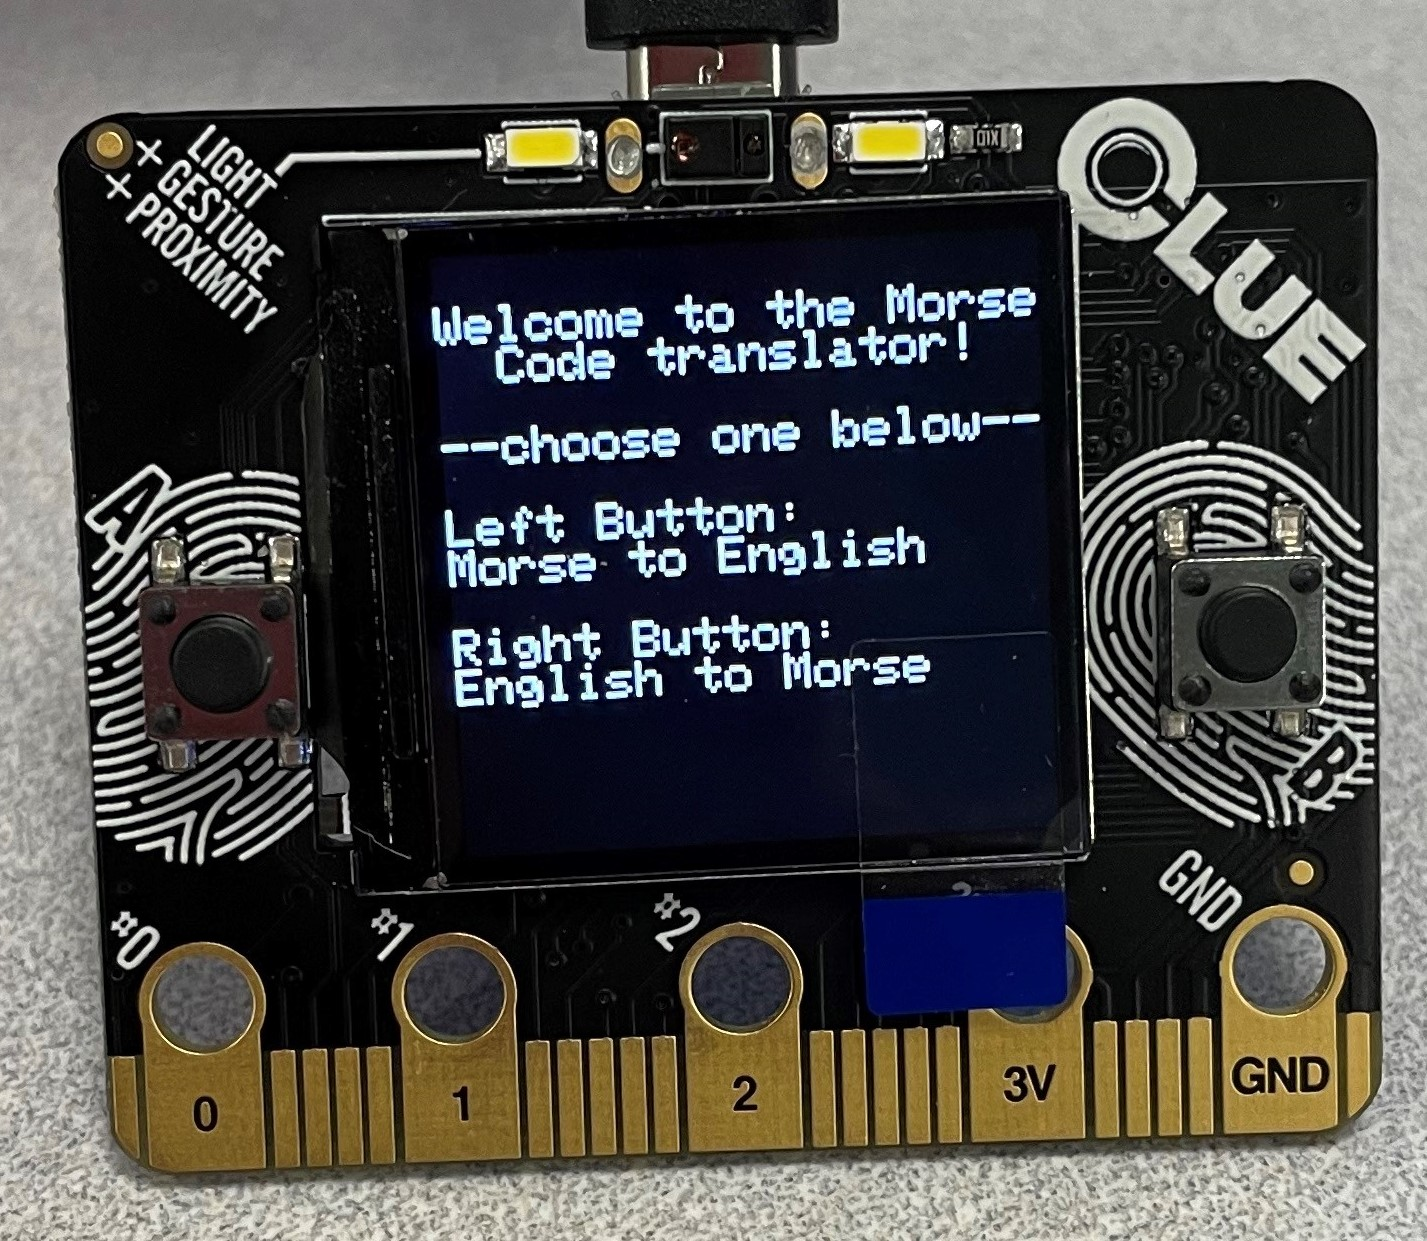
\includegraphics[width=4 in]{images/Main Screen.jpg}
\caption{Morse Code Translator Main Screen}
\label{Clueboard_mainmenu}
\end{figure}

Mediocre at Computers And Software (MCAS) is a group of individuals brought together through our common class, AERE 361. In the group, we have Ethan Schmidt the team lead, Burke Weber and Eric Rasmussen the Arduino and Clue board experts, Oda Natsuki as the C programmer, and Evan Kluch the debugger. Together this group created a Morse code translator that allows the user to translate either English to Morse or Morse to English.\\

\section{FEATURES}
The system is capable of completing the following tasks:\\
\\
Morse to English:\\
This setting allows you to input Morse code using the left and right buttons of the Clue board. 
After five seconds without inputs from the user, the Morse code is translated and displayed on the Clue board screen. If a Morse segment is entered that does not match anything in the library, it will skip over the segment and move on. \\
\\
English to Morse:\\
This setting allows a user to input a word or sentence on the computer keyboard via the serial port. The program will automatically translate the text into Morse, and will flash and beep the output on the Clue board. Since this is an infinite loop the user can continue to enter letters into the computer until they reset the clue board. \\
\\
User Interface:\\
The user interface is a display screen that allows the user to decide which way they would like to translate. This is the first screen that appears when turning on the translator. Once the mode is selected, the user interface will clear from the screen to allow use for other inputs and outputs to be displayed. \\

\section{PROBLEM STATEMENT}
Morse code was the first way of long-distance communication. Samuel Morse created it alongside the electrical telegraph, which it works hand in hand with. The creation of Morse Code was a pivotal moment in history, because it led to the development of modern communication. Although not as prevalent as it once was, the use of Morse code today is still critical to many. In addition to its recreational use in ham radios, its more critical role is in emergency communication signals and helping disabled individuals communicate more easily.\\
\\
A common use of Morse, SOS is the universal sign of distress that is used when situations go awry. People use SOS internationally when they find themselves in these unfortunate situations. It quite literally means “Save Our Souls”. This is why Morse code is still important to this day. Knowing how to signal to potential passersby that help is needed can potentially save lives.\\
\\
Morse code can be life-saving in critical situations, but it also can help people in their daily lives. Individuals that have medical disabilities or impairments have found the use of Morse code very helpful as a means of communication. For example, someone who is blind-deaf can translate a message in Morse code through the use of a device that produces small vibrations. This allows them to feel each “dit” and “dah” that make up the message. In another case, someone who has a speech impairment and does not have the ability to use sign language can use Morse code as their primary mode of communication. It is very clear that Morse code has a place in our modern world, even though the aforementioned cases represent a small minority.\\
\\
Based on the significance of Morse code’s uses, we believe that the language should be adopted by more people. If the skill of reading it, comprehending it, and responding coherently is more widespread across the globe, its usefulness will be exploited on more frequent occasions. Its capability to save someone’s life when they find themselves in a sticky situation makes it a useful tool to have in your back pocket. It’s also something that advantages individuals with disabilities or impairments. They appreciate its capability and enabling potential, even though most others find Morse code useful infrequently.\\
\\
Since we know that most people are unable to read or understand Morse code our goal is to create a way for people to learn the language through an interactive and straightforward system.\\
\\

\section{PROBLEM SOLUTION}
The Morse code translator we created is able to translate both from English to Morse, and from Morse to English. The program is built around the main void loop which runs continuously. Inside this loop is the User Interface and both the Morse-to-English and English-to-Morse main loops. The void loop can be seen in Appendix \ref{sourcecode}. The user is prompted to select which translation direction to use on the User Interface screen. By pressing either the left or right button, the user can enter the Morse-to-English translator or the English-to-Morse translator, respectively.\\

We began this project by creating libraries to translate to and from Morse code. This was the simplest task to complete first and it set us up well to achieve the rest of the tasks. The next major step was to learn how to take inputs and outputs from the Adafruit Clue Board.
\subsection{I/O in Arduino IDE}
Before starting this project, none of our team members had experience using Arduino IDE in any capacity. Because of this, there was a steep learning curve that we needed to overcome before we could begin any of the major programming. 
\subsubsection{Clue LCD Display}
The first I/O we attempted to learn was printing to the Clue board LCD display. This proved to be challenging to do on our own, so we referenced the Full Clue board Test \cite{ClueBoardTest} that printed the sensor data to the screen. This is the same program that was installed on the Clue board during its initial setup. This program was very helpful in teaching us how to print to the LCD display, and how to take button inputs. We also learned of many important libraries that are required for inputs and outputs on the Clue board. In order to print to the LCD display, we need to use the Arcada library and type \emph{arcada.display-$>$print("")} to display text in the quotes on the display. We also learned that the screen can display 20 characters per line, for a maximum of 14 lines with a text size of 2. Once we figured out how to print to the screen, we also deemed it important to learn how to clear the screen. We were not able to find a function that automatically clears the screen, so we created a for loop that prints 20 spaces per line, for 14 lines. After solving the problem of clearing the screen, the last thing to learn was how to print characters and automatically have the program skip to the next line if over the 20-character per-line limit. Again, we did not find a function that would do this for us automatically, so we created another for loop to accomplish this. This loop prints the current indexed element of a char array and continues to loop through for all of the elements. Another important feature is the if statement within the for loop. This will allow the characters to print on the next line if the number of characters is over 20. This if statement will repeat for every 20 characters so that the only thing limiting the number of lines we can print is the 14-line limit of the physical hardware. 
\subsubsection{Button Inputs}
The next thing to learn was how to take button inputs and how to create actions based on the buttons' inputs. Again, from the Full Clue Board Test \cite{ClueBoardTest}, we were able to learn how to do this. Using \emph{arcada.readbuttons()} we can read if a button is pressed and which button on the board was pressed, either the left button (button A), or the right button (button B). The left and right buttons can be seen on either side of the LCD display in Figure \ref{Clueboard_mainmenu}. From this, we can then use if statements to have the program do certain actions based on if the left button was pressed or if the right button was pressed. This will be important later on in our project when we need to implement this for navigating the user menu and inputting Morse code. 
\subsubsection{Serial Inputs}
The last main input/output to learn was taking English inputs from the Serial Monitor in Arduino IDE. The Serial Monitor environment is shown in Figure \ref{SerialMonitor}. While this seemed trivial to take inputs from the serial at first, it proved to be the hardest input or output to learn. While using the Serial Monitor, there is no function like \emph{fgets} in the C programming language that would allow us to directly store the user input into a character array. We initially tried to find functions that could accomplish this but found that we would not be able to read the entire input all at once. Rather, we found that we could read one character at a time from the Serial Monitor input. This idea came from doing outside research online. Specifically, the article \emph{Using Serial.read() with Arduino} by Michael James \cite{Serialreaddocumentation} was very helpful in learning how the \emph{Serial.read()} function works. \emph{Serial.read()} works by reading in the first character of the inputted string which can be stored into a char array, and then eliminating it from the string. If \emph{Serial.read()} is in a loop, such as one created by using \emph{while(Serial.available()}, then \emph{Serial.read()} will ultimately read through each character in the string until there are no characters left, at which point \emph{Serial.available()} will return a 0. We also found code online \cite{Serialreadingcode} to properly read serial inputs. This code was used as the basis for reading serial inputs in our program.

\begin{figure}[!ht]
\centering
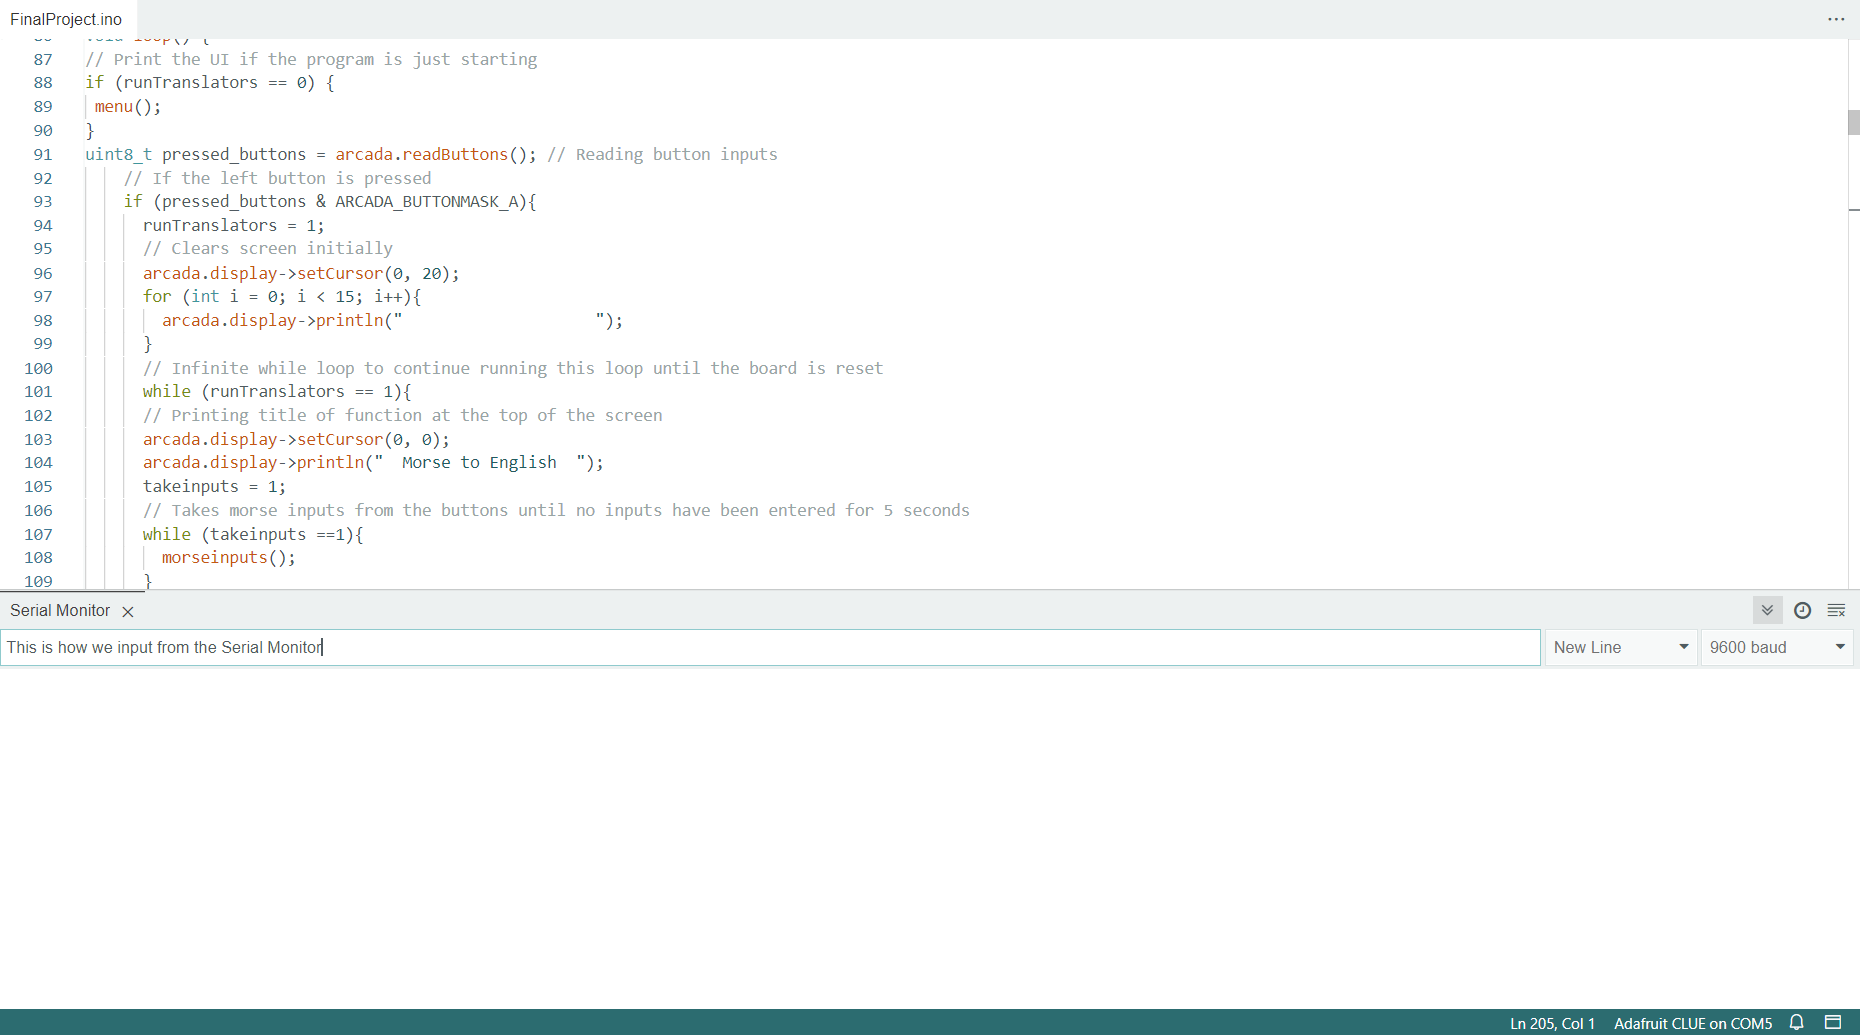
\includegraphics[width=5.5 in]{images/Serial Monitor.png}
\caption{Serial Monitor Environment}
\label{SerialMonitor}
\end{figure}

\FloatBarrier
\subsection{Program Design}
After we learned how to take inputs and outputs from the Clue board, we could begin designing the actual program. We learned that the best strategy would be to call other functions from outside the main loop into the main loop. By doing this, we could keep the main loop shorter and simpler and only call outside functions when they are needed, which also allows it to run faster. As the individual functions were developed, we found the best program design would be to have the User Interface as a separate function that is called at the start of the main loop. Then, if the left button is pressed while on the main menu, the program will go to the Morse-to-English translation mode. Or, if the right button is pressed while on the main menu, the program will go to the English-to-Morse translation mode. Figure \ref{Clueboard_mainmenu} from above, which shows the User Interface, is shown again below as Figure \ref{UserInterface}. Once we came up with the design for our program, we decided to work on one function at a time, beginning with the User Interface, then the English-to-Morse program, and finally the Morse-to-English program.

\begin{figure}[!ht]
\centering
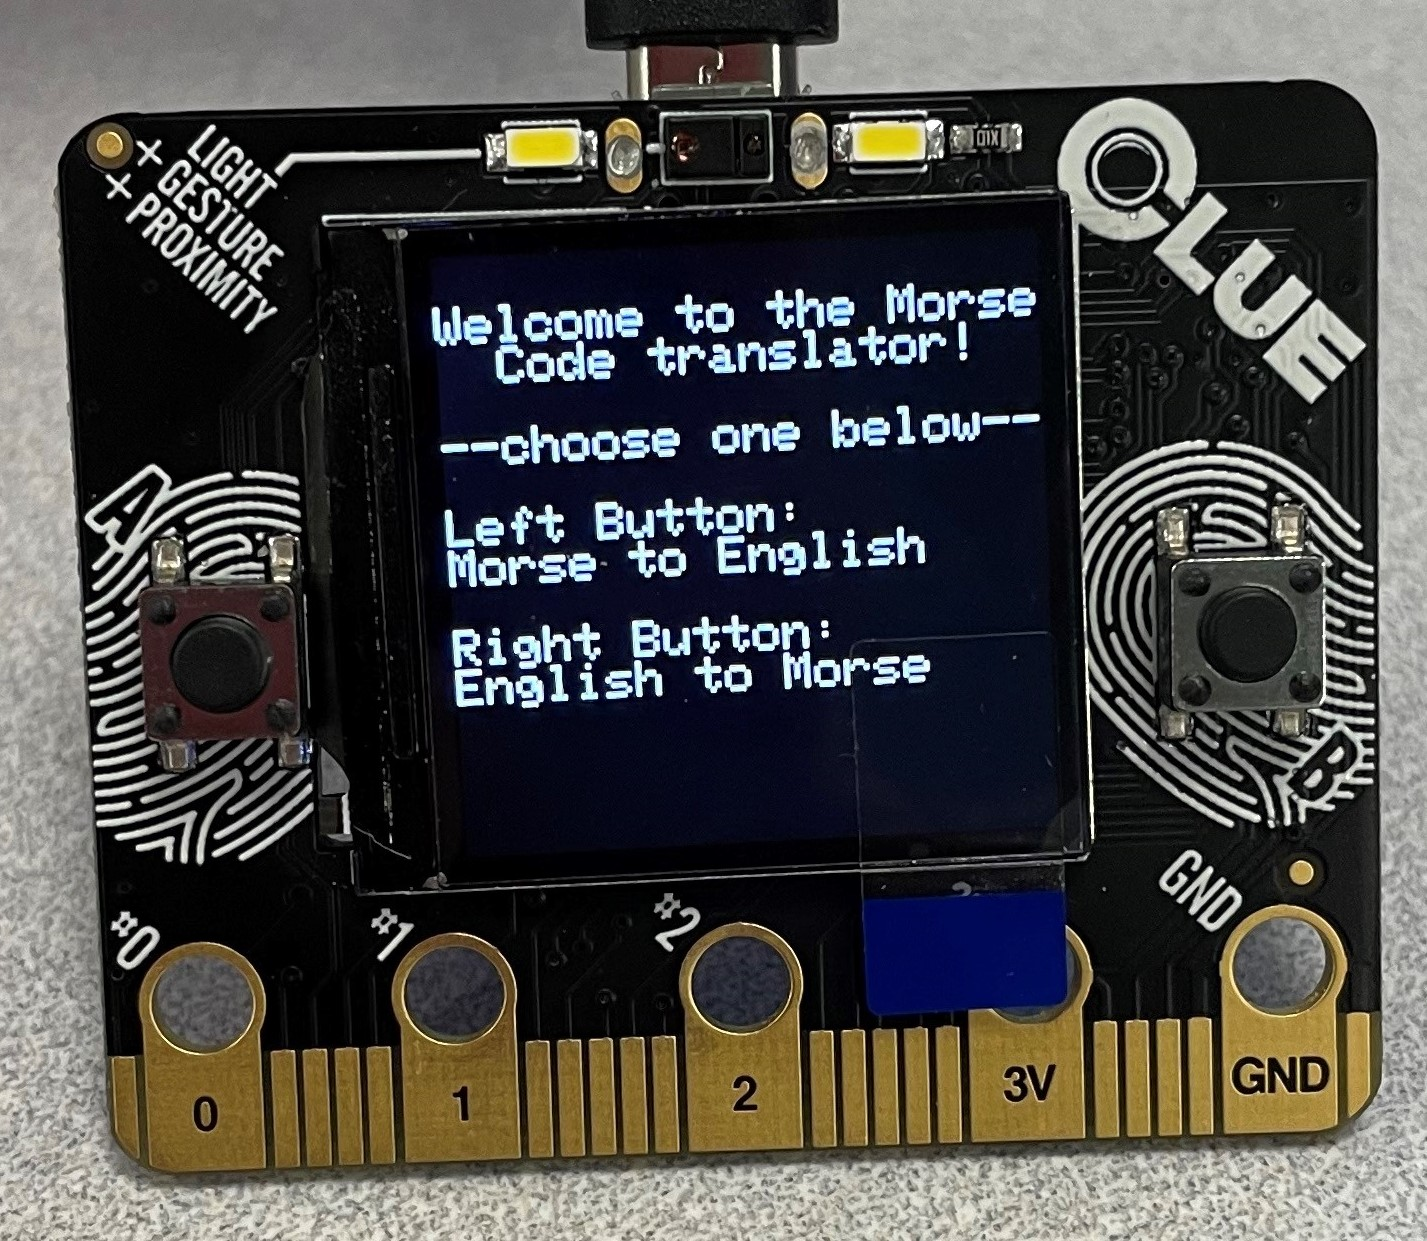
\includegraphics[width=4 in]{images/Main Screen.jpg}
\caption{Morse Code Translator Main Screen}
\label{UserInterface}
\end{figure}
\subsubsection{User Interface}
The user interface was probably the most simple function to write for our complete program. As mentioned before, we decided to keep the main features of our code written into functions, as this would make it easier to debug and stay organized overall. In the setup loop of our code, the Clue board's display is turned on by using the \emph{arcada.displayBegin()} command. So, in our menu function, all we had to do was set our text color and the initial position of the display's cursor. We chose to set the cursor on the left edge and 20 pixels below the top of the screen to allow for better centering of our menu. Once the Clue's display is turned on and the cursor position is set, we used a series of Arduino print statements in order to display the menu. The \emph{arcada.display} commands in Arduino were useful to us since we included the library in our setup code. The \emph{printLn} arcada display command is what we used to print text, then go to a new line. If we wanted to print a blank line, we simply put five spaces in the parenthesis instead of text. Using just \emph{print} prints text, but doesn't go to the next line afterward. It only took a few commands to display our menu.\\
\\
The reason we chose this method to display a menu is that our program does not require a complex one by any means. There are only two translator options that the user has to choose from. We also only have one location where the menu needs to be displayed for the user to interact with. It is when the user initially starts the program, and when they want to switch over to the other translator. Because of this, we did not need to call the menu function in our code anywhere else than at the beginning of our program. If the user wants to return to the menu so that they can restart the current translator they are on, or so they can choose the other one, all they have to do is press the reset button on the back of the Clue board. Our code takes milliseconds to reboot on the board, so the menu will reprint right away after the reset button is pressed. The reset button can be pressed at any time while the program is running, allowing the user to exit each translator with ease at any point in time.\\
\\
The user interface is a very simple way to guide our users to the necessary translation method. It welcomes them to the program and prompts them with a button press to select Morse to English or English to Morse. Our user interface makes the whole program very easy to use. Since we didn't implement any external sensors or buttons - other than a phone or laptop as the program's serial monitor - the program is not difficult to maneuver at all. There are only two buttons that can be pressed for operation and an additional one for resetting the program. Its simplicity adds to its effectiveness because the user will not have to learn how to use the device and program. Instead, they will be able to allocate all of their focus on actually using the translators and practicing their skills to learn Morse code.
\FloatBarrier
\subsubsection{English to Morse}
By pressing the right button while on the User Interface main screen, the user will enter the English-to-Morse translator. Once in the program, the screen will clear and print the title of the translation function the user is currently in. This is shown in Figure \ref{EtoM}. Then, an infinite loop will starts that can only be broken by resetting the Clue board with the button on the back. Inside this loop, a series of outside functions will be called to accomplish the translation. The first is the \emph{readinput()} function, which reads in the English input using \emph{Serial.read()} and calls the English-to-Morse library \emph{EtoM} to translate each new input character to Morse code. Each English character is stored in a char array called \emph{latinText}, and the string of Morse characters is stored in a char array called \emph{morse}. Once all the characters have been read and translated, a logic variable is set to 1 at the end of \emph{readinput()} and the program returns to the infinite while loop in the English to Morse section of the main loop. The next function called is the \emph{showNewInput} function. This function will print English characters and Morse characters to the Serial Monitor while also printing the English Characters to the Clue board display. The \emph{showNewInput} function will only print the latinText and morse char arrays if a new input has been entered in by the user due to the logic variable set to 1 in \emph{readinput()}. Once the input has been printed, the last function called is the \emph{buzzer} function which outputs the Morse code on the Clue board using the speaker and the LED. The buzzer and LED output simultaneously which provides the user the best chance of picking up the outputted signals. The output of the Morse code is set to 20 words per minute, which is very fast for a new user, but is average for an experienced user. The timing between characters is as follows:
\begin{itemize}
    \item Dot length: 60 milliseconds
    \item Dash length: 180 milliseconds
    \item Time between Morse characters (dot or dash): 60 milliseconds
    \item Time between English characters: 180 milliseconds
    \item Time between English words: 420 milliseconds
\end{itemize}
Once all of the functions have been called, the \emph{latinText} and \emph{morse} char arrays are reset to 0s so that the user can then make new inputs to translate. The user can make an infinite amount of inputs that are each less than 280 English characters. If the user wishes to exit the program, they can press the reset button on the back of the Clue board to return to the main menu.
\begin{figure}[!ht]
\centering
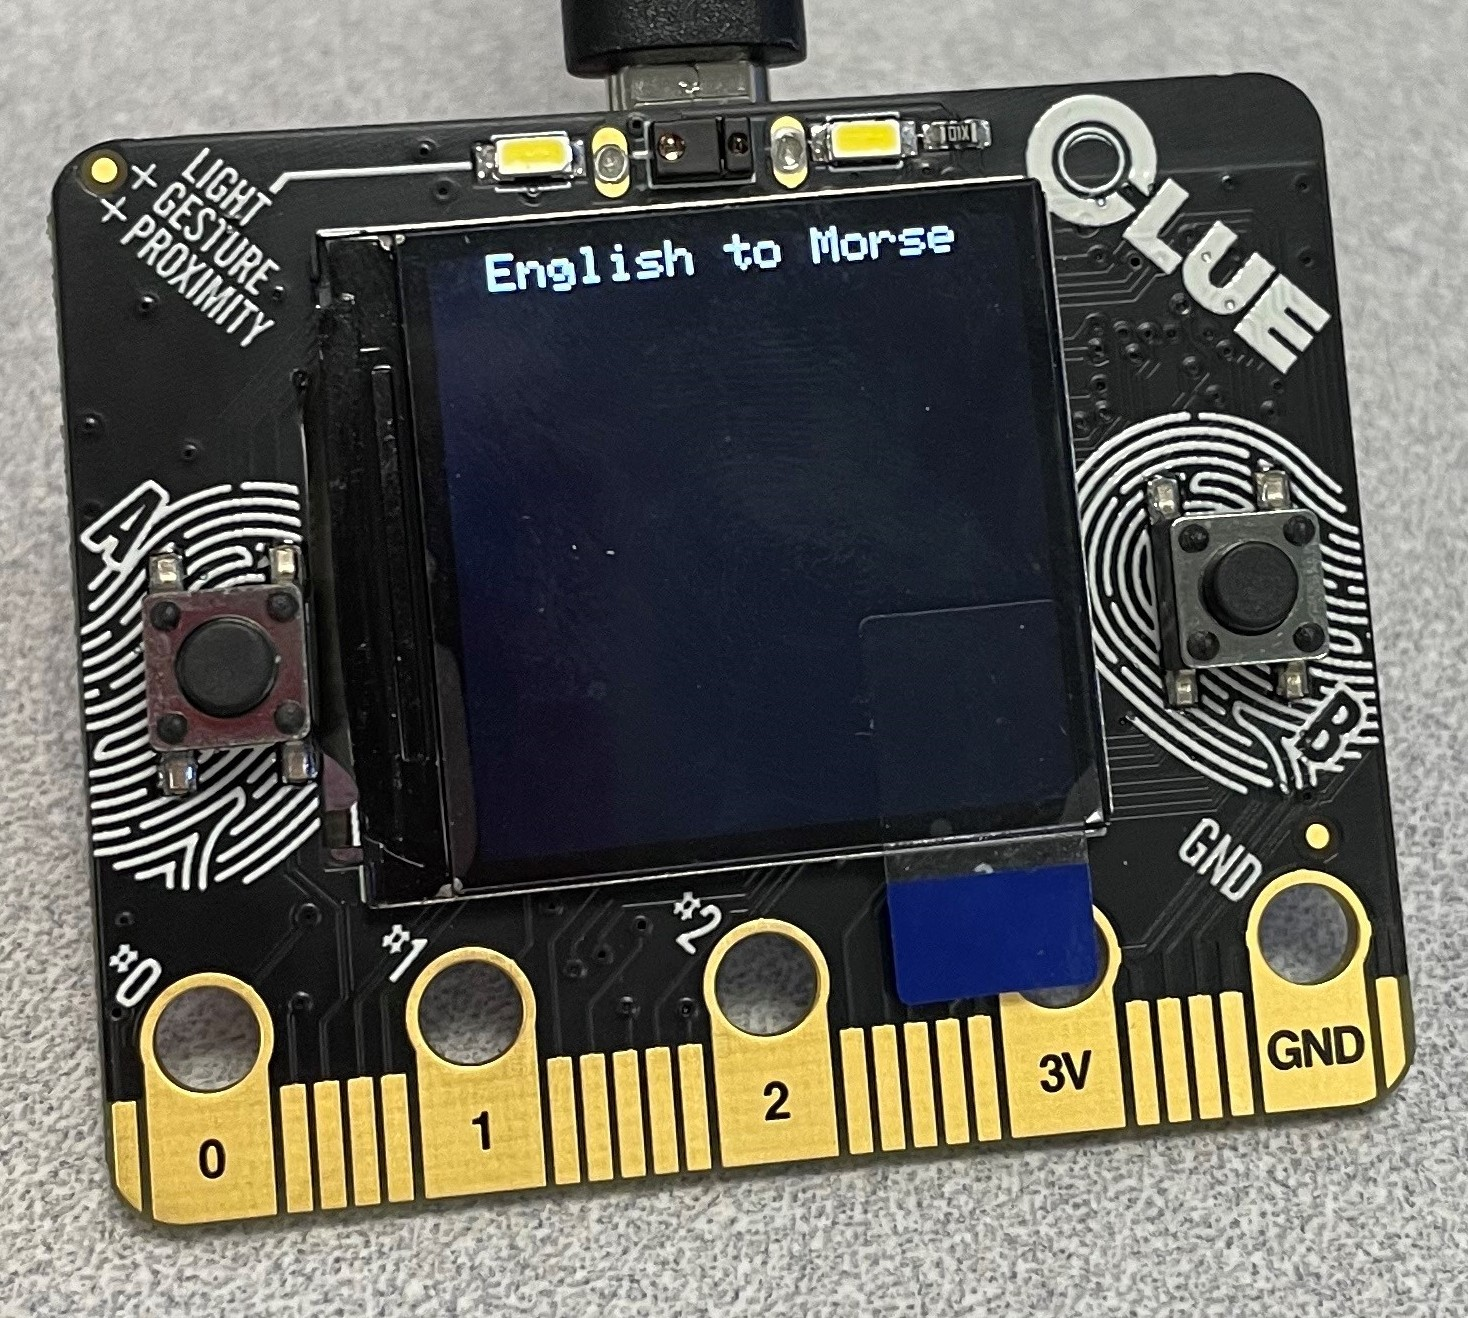
\includegraphics[width=4 in]{images/EtoM.jpg}
\caption{English to Morse Main Screen}
\label{EtoM}
\end{figure}

\FloatBarrier
\subsubsection{Morse to English}
By pressing the left button while on the User Interface main screen, the user will enter the Morse-to-English translator. Once in the program, the screen will clear and print the title of the translation function the user is currently in. This is shown in Figure \ref{MtoE}. Then, an infinite loop will starts that can only be broken by resetting the Clue board with the button on the back. Inside this loop, a series of outside functions will be called to accomplish the translation. The first function called is \emph{morseinputs} which takes in the button inputs as Morse code. This function is called specially, as it is continuously called within a nested while loop that runs infinitely. The only way to break this inner loop, and to stop calling \emph{morseinputs}, is to not give a Morse input for 5 seconds. Inside this \emph{morseinputs} function, the program reads which button is pressed. Two if statements determine that if the left button is pressed, either a dot or a dash will be inputted into the \emph{morse} char array, and if the right button is pressed, either an end-of-character space or an end-of-word space will be inputted into the \emph{morse} char array. To determine whether the user inputs a dot or dash, or an end-of-character or end-of-word, the program users timer variables. When the button is first pressed, the time in the program is recorded using \emph{millis()}. Then, an infinite loop is created that reads the button input and runs while there is still a button input, essentially pausing the program while the button is being pressed. Once the button is let go of, the time in the program is again recorded. The difference between the time the button was released and the time the button was first pressed is then calculated. The time-character relation for each button is shown below.\\
For the left button, the following characters will be added to the \emph{morse} char array based on the time the button is held for.
\begin{itemize}
    \item Less than 150 milliseconds: dot
    \item Morse than 150 milliseconds: dash
\end{itemize}
For the right button, the following characters will be added to the \emph{morse} char array based on the time the button is held for.
\begin{itemize}
    \item Less than 150 milliseconds: New English character space
    \item More than 150 milliseconds: New English word space
\end{itemize}
Then, the inputted character will be displayed on the Clue board screen. Finally, the time at the end of the function is recorded. If the current time minus the time since the last button input is more than 5 seconds, then the while loop continuously calling \emph{morseinputs} will break and the next functions can be called. After \emph{morseinputs} function completes, the \emph{translateMtoE} function is called to translate the Morse code to English text. This function works by finding the spaces between characters (a less than 150-millisecond press of the right button) and splitting the char array at these points. Then, the individual char arrays can be compared to the Morse-to-English library and translated to English text stored in the \emph{latinText} array. Once the text is translated, the \emph{showNewInput} function is called and it works the same as in the English-to-Morse translator. This time, the translated text is the English text that appears on the Clue board display. Finally, the \emph{latinText} and \emph{morse} char arrays are reset to 0s so that the user can then make new inputs to translate. The user can again make an infinite number of inputs but is limited to 1500 Morse characters per translation which is due to the estimated number of Morse characters for the maximum number of English characters that can be displayed on the screen.

\begin{figure}[!ht]
\centering
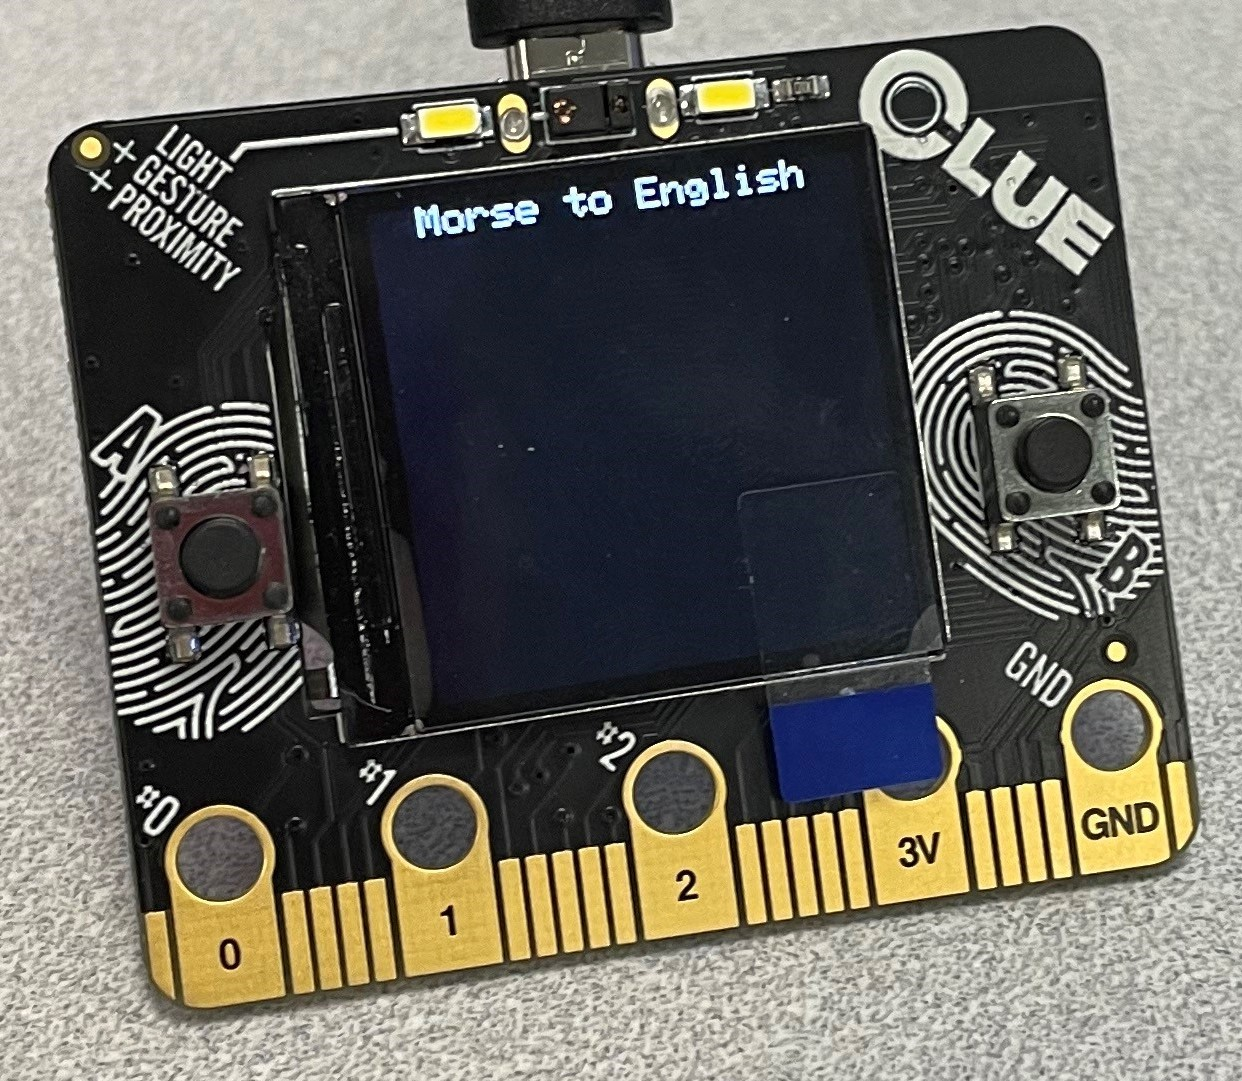
\includegraphics[width=4 in]{images/MtoE.jpg}
\caption{Morse to English Main Screen}
\label{MtoE}
\end{figure}

\FloatBarrier

\subsubsection{Library of Characters}
The library of characters is structured in an if-else statement, serving as a reference for incoming strings. The library uses string comparison to detect matches between the input segment and the library and prints the corresponding translation. If a match isn't found, it skips over the input segment and moves on to the next, and does not warn the user that the segment couldn't be translated.

The library is shown below, and the code to implement the library is below that.
\begin{figure}
    \centering
    \caption{Table 1 Character and its American Morse Code(AMC)}
    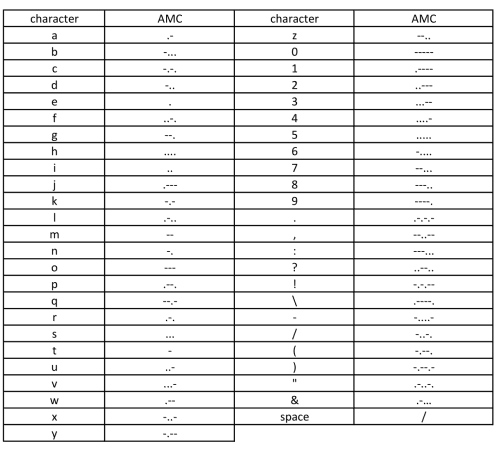
\includegraphics[width=6 in]{images/table-1.png}
    \label{fig:AMCtable}
\end{figure}
\\ \\ \\ \\

\begin{lstlisting}[language=Arduino]
# function for translating from english to morse
if (c == 'A' || c == 'a') {
        strcat(morse,".- ");
    }
    else if (c == 'B' || c == 'b') {
        strcat(morse,"-... ");
    }
    else if (c == 'C' || c == 'c') {
        strcat(morse,"-.-. ");
    }
    else if (c == 'D' || c == 'd') {
        strcat(morse,"-.. ");
    }
    else if (c == 'E' || c == 'e') {
        strcat(morse,". ");
    }
    else if (c == 'F' || c == 'f') {
        strcat(morse,"..-. ");
    }
    else if (c == 'G' || c == 'g') {
        strcat(morse,"--. ");
    }
    else if (c == 'H' || c == 'h') {
        strcat(morse,".... ");
    }
    else if (c == 'I' || c == 'i') {
        strcat(morse,".. ");
    }
    else if (c == 'J' || c == 'j') {
        strcat(morse,".--- ");
    }
    else if (c == 'K' || c == 'k') {
        strcat(morse,"-.- ");
    }
    else if (c == 'L' || c == 'l') {
        strcat(morse,".-.. ");
    }
    else if (c == 'M' || c == 'm') {
        strcat(morse,"-- ");
    }
    else if (c == 'N' || c == 'n') {
        strcat(morse,"-. ");
    }
    else if (c == 'O' || c == 'o') {
        strcat(morse,"--- ");
    }
    else if (c == 'P' || c == 'p') {
        strcat(morse,".--. ");
    }
    else if (c == 'Q' || c == 'q') {
        strcat(morse,"--.- ");
    }
    else if (c == 'R' || c == 'r') {
        strcat(morse,".-. ");
    }
    else if (c == 'S' || c == 's') {
        strcat(morse,"... ");
    }
    else if (c == 'T' || c == 't') {
        strcat(morse,"- ");
    }
    else if (c == 'U' || c == 'u') {
        strcat(morse,"..- ");
    }
    else if (c == 'V' || c == 'v') {
        strcat(morse,"...- ");
    }
    else if (c == 'W' || c == 'w') {
        strcat(morse,".-- ");
    }
    else if (c == 'X' || c == 'x') {
        strcat(morse,"-..- ");
    }
    else if (c == 'Y' || c == 'y') {
        strcat(morse,"-.-- ");
    }
    else if (c == 'Z' || c == 'z') {
        strcat(morse,"--.. ");
    }
    else if (c == '0') {
        strcat(morse,"----- ");
    }
    else if (c == '1') {
        strcat(morse,".---- ");
    }
    else if (c == '2') {
        strcat(morse,"..--- ");
    }
    else if (c == '3') {
        strcat(morse,"...-- ");
    }
    else if (c == '4') {
        strcat(morse,"....- ");
    }
    else if (c == '5') {
        strcat(morse,"..... ");
    }
    else if (c == '6') {
        strcat(morse,"-.... ");
    }
    else if (c == '7') {
        strcat(morse,"--... ");
    }
    else if (c == '8') {
        strcat(morse,"---.. ");
    }
    else if (c == '9') {
        strcat(morse,"----. ");
    }
    else if (c == '.') {
        strcat(morse,".-.-.- ");
    }
    else if (c == ',') {
        strcat(morse,"--..-- ");
    }
    else if (c == ':') {
        strcat(morse,"---... ");
    }
    else if (c == '?') {
        strcat(morse,"..--.. ");
    }
    else if (c == '\'') {
        strcat(morse,".----. ");
    }
    else if (c == '-') {
        strcat(morse,"-....- ");
    }
    else if (c == '/') {
        strcat(morse,"-..-. ");
    }
    else if (c == '(') {
        strcat(morse,"-.--. ");
    }
    else if (c == ')') {
        strcat(morse,"-.--.- ");
    }
    else if (c == '"') {
        strcat(morse,".-..-. ");
    }
    else if (c == '&') {
        strcat(morse,".-... ");
    }
    else if (c= ' ') {
        strcat(morse,"/  ");
    }
    return morse;
}

// Morse to English library
// Compares Morse input characters to the library, then assigns corresponding English character to the latintext array
char* MtoE(char* segment,char* output) {
    if (strcmp(segment,".-") == 0) {
        strcat(output,"a");
    }
    else if (strcmp(segment,"-...") == 0) {
        strcat(output,"b");
    }
    else if (strcmp(segment,"-.-.") == 0) {
        strcat(output,"c");
    }
    else if (strcmp(segment,"-..") == 0) {
        strcat(output,"d");
    }
    else if (strcmp(segment,".") == 0 && strlen(segment) == 1) {
        strcat(output,"e");
    }
    else if (strcmp(segment,"..-.") == 0) {
        strcat(output,"f");
    }
    else if (strcmp(segment,"--.") == 0) {
        strcat(output,"g");
    }
    else if (strcmp(segment,"....") == 0) {
        strcat(output,"h");
    }
    else if (strcmp(segment,"..") == 0 && strlen(segment) == 2) {
        strcat(output,"i");
    }
    else if (strcmp(segment,".---") == 0) {
        strcat(output,"j");
    }
    else if (strcmp(segment,"-.-") == 0) {
        strcat(output,"k");
    }
    else if (strcmp(segment,".-..") == 0) {
        strcat(output,"l");
    }
    else if (strcmp(segment,"--") == 0) {
        strcat(output,"m");
    }
    else if (strcmp(segment,"-.") == 0) {
        strcat(output,"n");
    }
    else if (strcmp(segment,"---") == 0) {
        strcat(output,"o");
    }
    else if (strcmp(segment,".--.") == 0) {
        strcat(output,"p");
    }
    else if (strcmp(segment,"--.-") == 0) {
        strcat(output,"q");
    }
    else if (strcmp(segment,".-.") == 0) {
        strcat(output,"r");
    }
    else if (strcmp(segment,"...") == 0) {
        strcat(output,"s");
    }
    else if (strcmp(segment,"-") == 0) {
        strcat(output,"t");
    }
    else if (strcmp(segment,"..-") == 0) {
        strcat(output,"u");
    }
    else if (strcmp(segment,"...-") == 0) {
        strcat(output,"v");
    }
    else if (strcmp(segment,".--") == 0) {
        strcat(output,"w");
    }
    else if (strcmp(segment,"-..-") == 0) {
        strcat(output,"x");
    }
    else if (strcmp(segment,"-.--") == 0) {
        strcat(output,"y");
    }
    else if (strcmp(segment,"--..") == 0) {
        strcat(output,"z");
    }
    else if (strcmp(segment,"-----") == 0) {
        strcat(output,"0");
    }
    else if (strcmp(segment,".----") == 0) {
        strcat(output,"1");
    }
    else if (strcmp(segment,"..---") == 0) {
        strcat(output,"2");
    }
    else if (strcmp(segment,"...--") == 0) {
        strcat(output,"3");
    }
    else if (strcmp(segment,"....-") == 0) {
        strcat(output,"4");
    }
    else if (strcmp(segment,".....") == 0) {
        strcat(output,"5");
    }
    else if (strcmp(segment,"-....") == 0) {
        strcat(output,"6");
    }
    else if (strcmp(segment,"--...") == 0) {
        strcat(output,"7");
    }
    else if (strcmp(segment,"---..") == 0) {
        strcat(output,"8");
    }
    else if (strcmp(segment,"----.") == 0) {
        strcat(output,"9");
    }
    else if (strcmp(segment,".-.-.-") == 0) {
        strcat(output,".");
    }
    else if (strcmp(segment,"--..--") == 0) {
        strcat(output,",");
    }
    else if (strcmp(segment,"---...") == 0) {
        strcat(output,":");
    }
    else if (strcmp(segment,"..--..") == 0) {
        strcat(output,"?");
    }
    else if (strcmp(segment,".----.") == 0) {
        strcat(output,"\'");
    }
    else if (strcmp(segment,"-....-") == 0) {
        strcat(output,"-");
    }
    else if (strcmp(segment,"-..-.") == 0) {
        strcat(output,"/");
    }
    else if (strcmp(segment,"-.--.") == 0) {
        strcat(output,"(");
    }
    else if (strcmp(segment,"-.--.-") == 0) {
        strcat(output,")");
    }
    else if (strcmp(segment,".-..-.") == 0) {
        strcat(output,"\"");
    }
    else if (strcmp(segment,".-...") == 0) {
        strcat(output,"&");
    }
    else if (strcmp(segment,"/") == 0) {
        strcat(output," ");
    }
    return output;
}
\end{lstlisting}

\subsection{Problem Solution Testing}
In the process of testing our code, there were two big issues with translating from Morse to English. At first, we are trying to conduct interpretation by another method which is not the same as the one we adopted finally. But in the test of that, it failed to print out and garbled characters appeared. So, we chose the \emph{strtok} function, which is used to separate each Morse code for translating process. American Morse Code is constructed by dot, dash, and one space to express each English character and symbol, so to make messages with fewer types of characters in Morse code, we first adopted double spaces to divide whole sentences in each Morse code that express a letter. When we set this function into the program and run a test, it failed because of the rule of the \emph{strtok} function that only one letter is allowed to use as a separating letter; Using double spaces is not allowable. For solving this issue, we have adopted another type of American Morse code that can express only by dot and dash into our program, and also we applied one space as the separate letter stored in \emph{strtok} function as an argument. Those settings are used in the final version of the translation program that works correctly.
\subsection{Problem Solution Reflection}
    We have checked if the program works correctly by translating Morse codes that express all alphabetical characters and numbers to English. First of all, we typed all alphabetical characters and numbers by keyboard to translate to Morse code, then input the Morse code retrieved in English to Morse process, and confirm whether the resulting output on the screen is the same as the user typed. Confirming if all symbols would be translated from Morse code to English is the same as the previous method. 
\subsection{Problem Solution in Action}

\begin{figure}[!t]
\centering
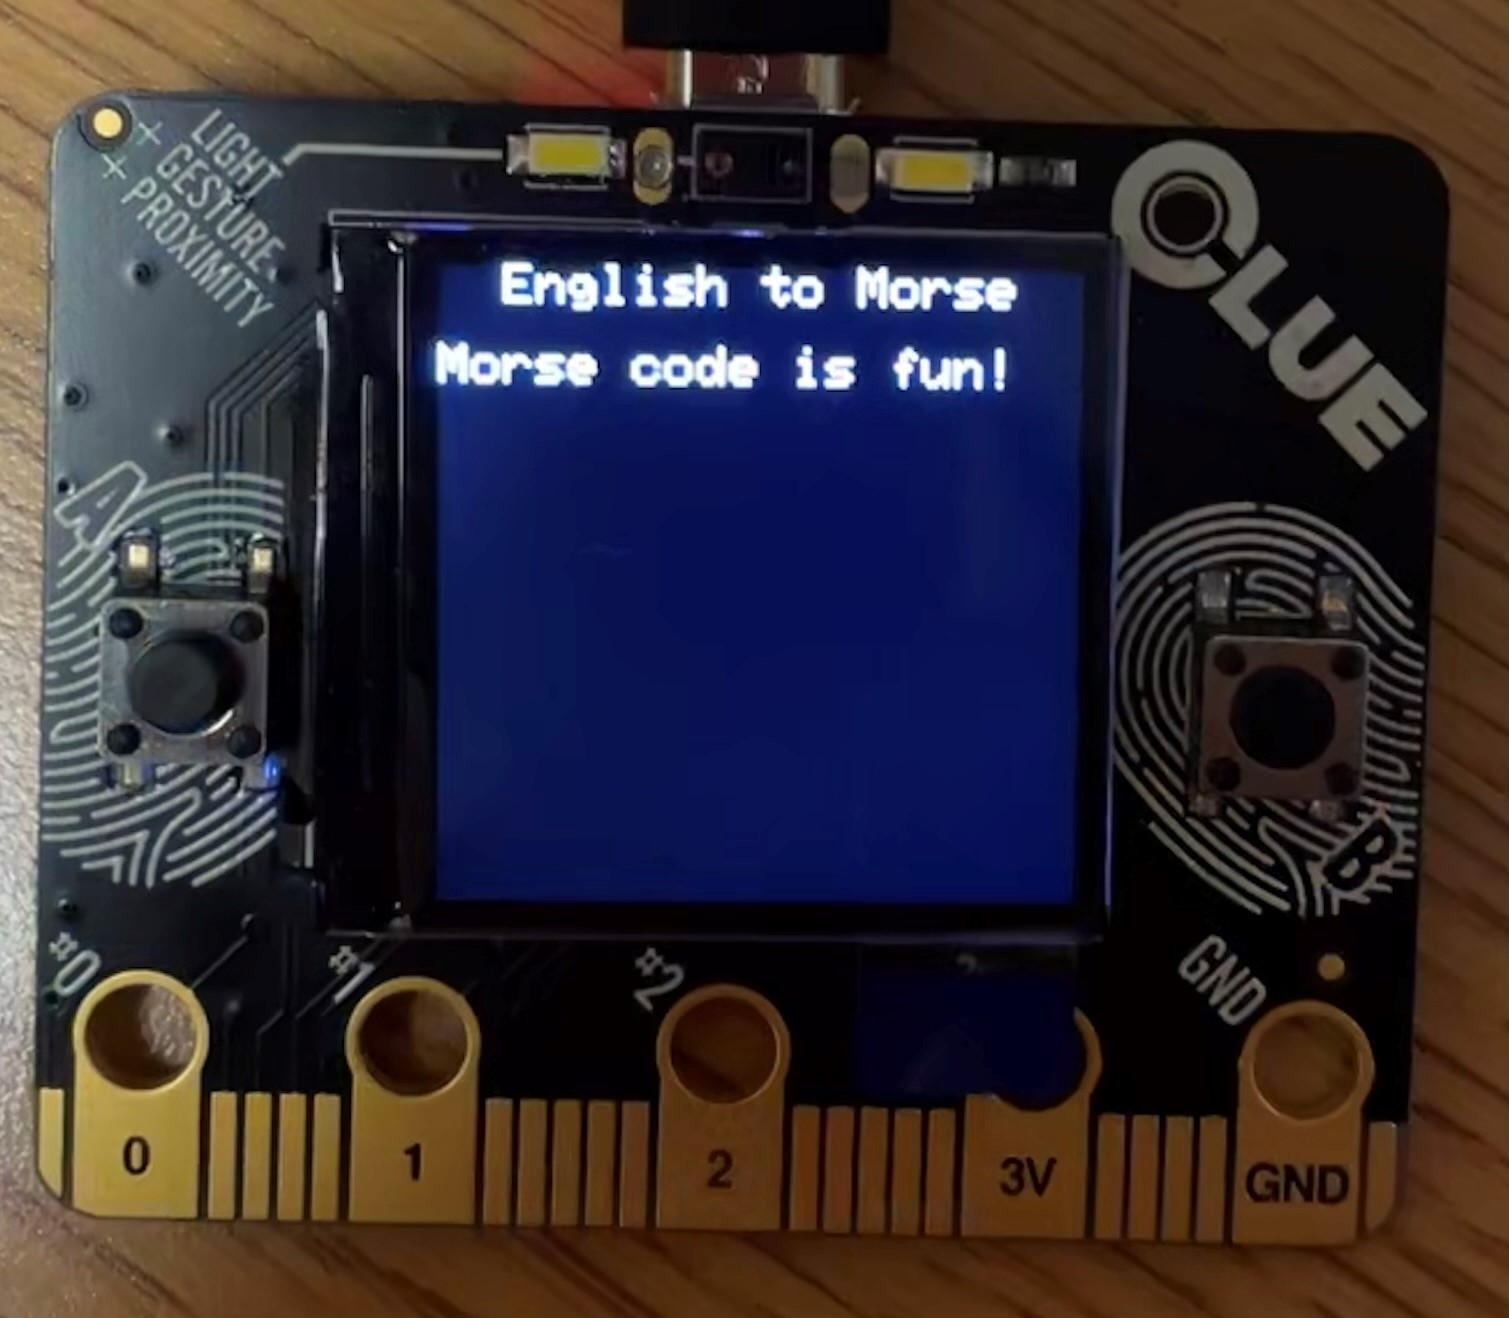
\includegraphics[width=4 in]{EtoMaction.jpg}
\caption{English to Morse output between flashes}
\label{fig:EtoMblank}
\end{figure}

\begin{figure}[!t]
\centering
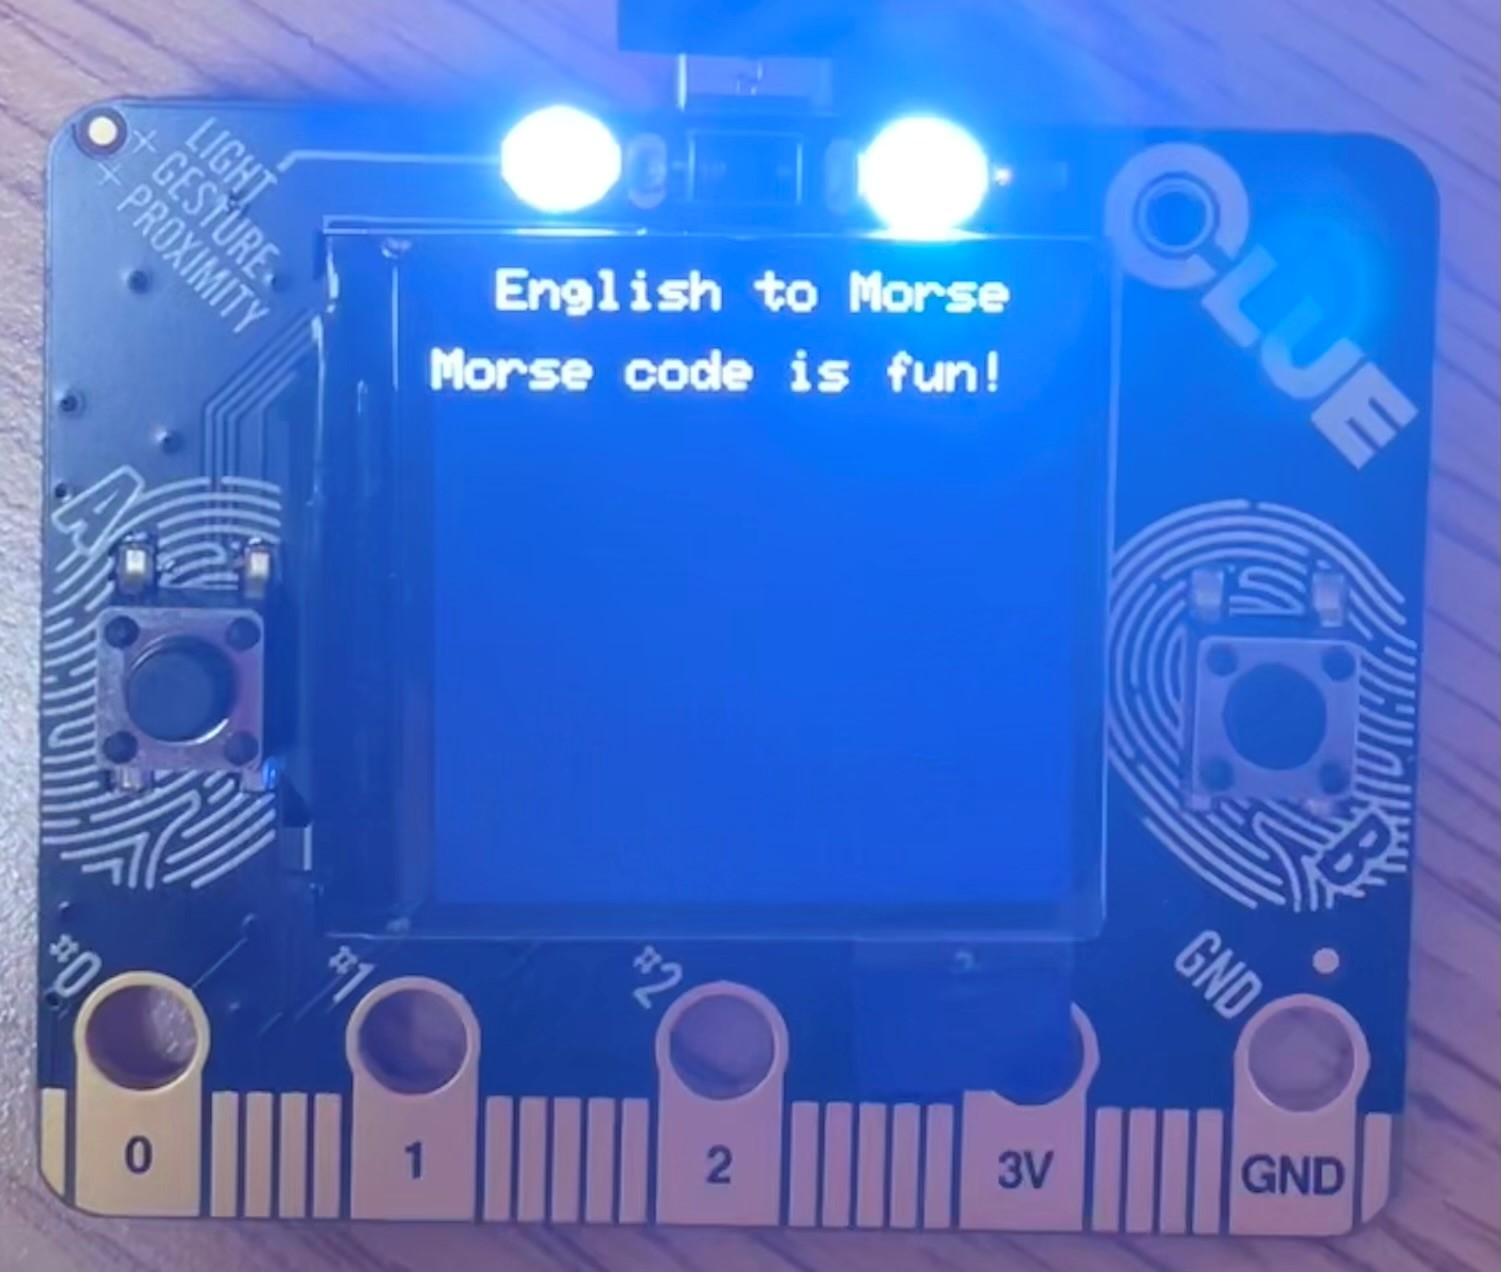
\includegraphics[width=4 in]{images/EtoMactionflash.jpg}
\caption{English to Morse output during flash}
\label{fig:EtoMflash}
\end{figure}

\begin{figure}[!t]
\centering
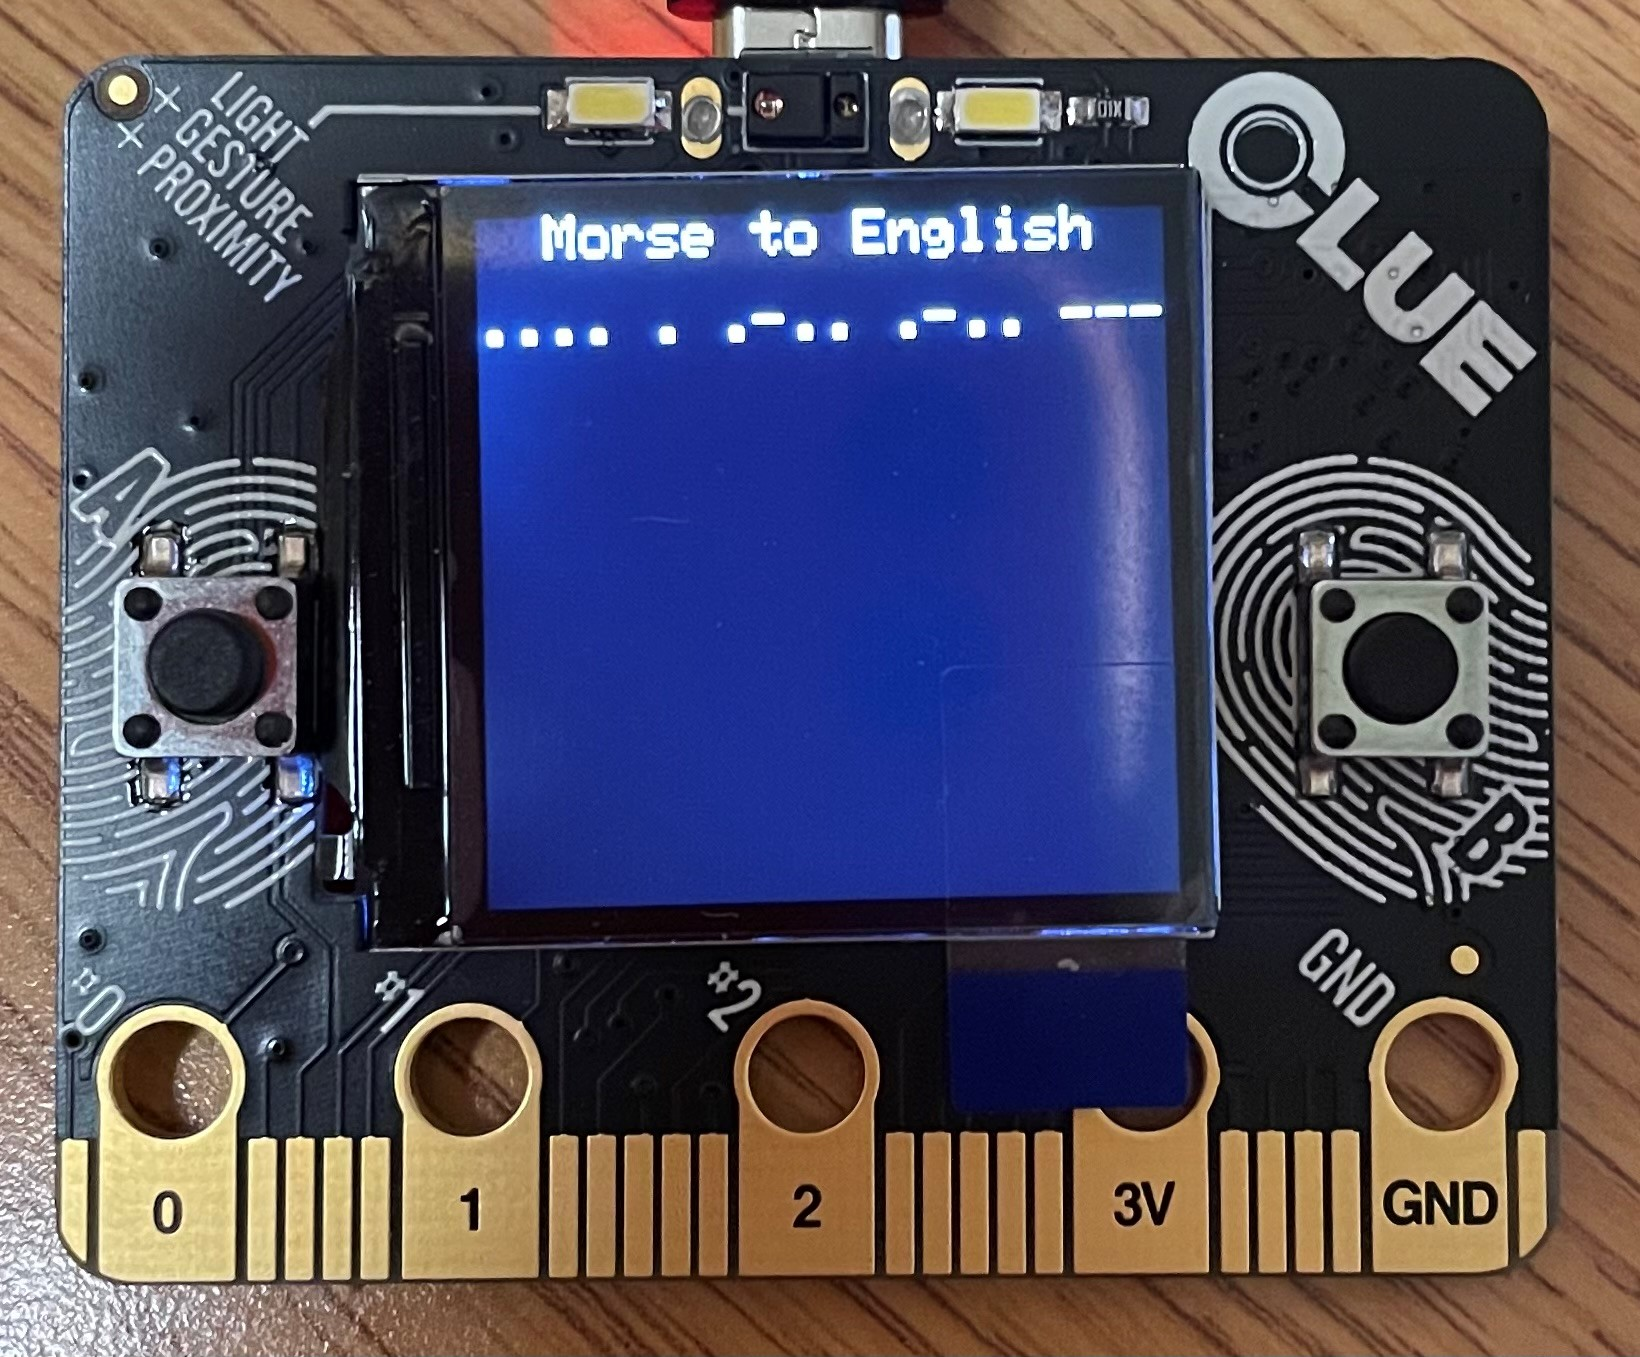
\includegraphics[width=4 in]{MtoEM.jpg}
\caption{Morse to English displaying inputted Morse code}
\label{fig:MtoEM}
\end{figure}

\begin{figure}[!t]
\centering
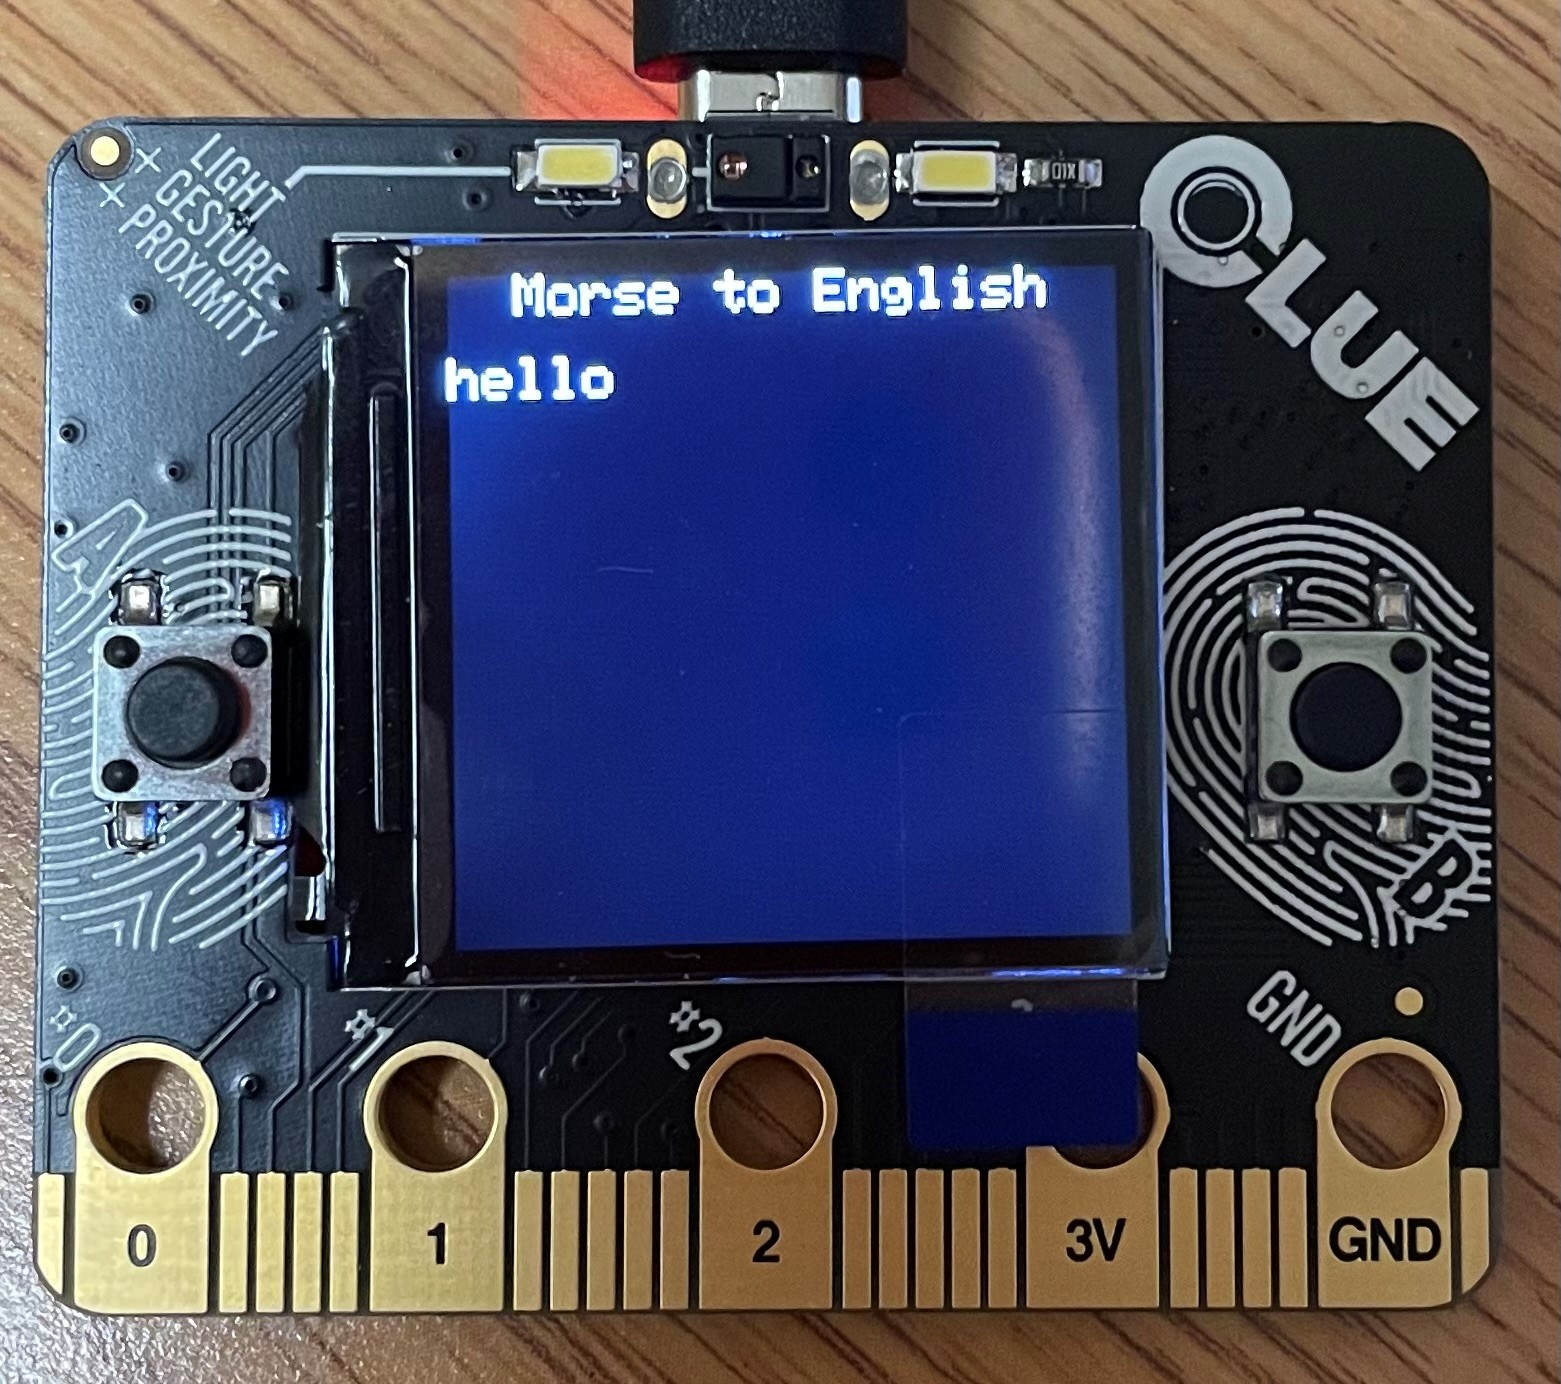
\includegraphics[width=4 in]{MtoEE.jpg}
\caption{Morse to English displaying English Translation}
\label{fig:MtoEE}
\end{figure}



\FloatBarrier
\section{STATUS}
Overall we believe that this project was done very successfully and the translator works as we wanted it to. When comparing it back with the goals described in the project proposal, we were able to not only complete all goals but went above and beyond with the ability to input multiple words. Initially, we were going to use one button for dots and the other for dashes which would have limited us in characters. However, since we found a way to use a timer to read the time the button was pressed, we were able to make the buttons more like normal Morse code which allowed us to incorporate more features. Beyond that, we understand that there are plenty of further developments that would make this system superior to where it is right now. This is discussed later in the report.\\
\\
\subsection{Lessons Learned}
As a group, we had the ability to work together on a project that was very new to all of us. Since this is the first time any of us were exposed to Arduino IDE, we clearly needed to learn how to write programs in the language. Furthermore, we learned more about the interactions of hardware and software as we looked into the code to make the lights flash and the speaker beep. Together as a team, we had to learn how to operate GitHub without the normal setup of teacher and student interaction. This meant that we could create and actually merge pull requests from fellow team members. Therefore, this project pushed us to learn how to cooperate like a team working in the industry because we had to organize all of our work with each other. Finally, we continued to work on our presentation, teamwork, and coding skills that have been developed in other classes.\\
\\
\section{RESULTS}
The embedded system we designed does not collect and store any data. The program is designed to translate the inputted Morse code or English text, then delete the data to translate another message. While letting others use the board, we found that there is a small bug in the code that causes a delay when typing in additional messages into the Morse to English translator. After the first message is translated, another message can be inputted in Morse code using the buttons to translate again. The issue we found is that the first button press is slightly delayed, by about half a second to a second longer than normal, but all of the following button presses will input the correct character right away. This is likely due to some extra code that needs to run to clear the screen before the program is ready to accept button inputs. In the future, we would use button callbacks to eliminate this bug and to make the program run more smoothly overall. When others used the Clue board to input a message in Morse, they found it difficult to work with the 150 millisecond time interval for dots and spaces between characters on the left and right buttons respectively. The 20 words per minute output speed was also difficult for some to keep up with, which makes it harder to learn with the program we created.

The source code that runs the Morse code translator is found in Appendix \ref{sourcecode}.

\section{FUTURE WORK}
If we were able to continue this project into the future there would be a couple more modes we would like to add to the system. we would keep the same main user interface, however, if you select the English to Morse translator we would like to incorporate a speed setting. Currently, the board is set to output at 20 words per minute which is very quick for someone who doesn't know Morse code. To make this system easy to learn, we would create slow and medium-speed settings as well. The code for this would be very easy to do as all that would change would be how long is needed for a dash vs a dot. Another useful capability for the translator to have would be a way to store all strings or characters that were unable to be translated properly, and print them after the translation was complete. For example, if the following Morse string was inserted: $$...-..$$ The following output would look like:
$$\text{Unable to translate Morse string "...-.."}$$Another setting we could implement is a training mode where the screen prints a letter and the user then has to input the Morse code for that letter. If the input is correct the screen would print a victory message and if not it would allow you to retry. This same idea could be used to learn words as a whole.\\
\\
\section{CONCLUSION}
In conclusion, MCAS was able to create a working Morse code translator. This system works using a library of stored characters and their corresponding Morse code translation. Then, in either English or Morse code, it compares each letter translating one letter at a time and storing it into a new character array. Finally, the translation is printed out either on the board or in a flashy fashion. This translator allows a user to learn Morse code or simply translate a message they see. \\
\\
Link to GitHub repository: \begin{verbatim}
    https://github.com/SomethingAboutBears/MCAS-Final-Project
\end{verbatim}
\newpage

\bibliographystyle{plain}
\bibliography{ref}
\newpage
% you need to have at least your code in your appendix
\appendix

\section{SOURCE CODE}
\label{sourcecode}
\lstinputlisting[language=Arduino]{src/FinalProject.ino}
\end{document}
